\def\name{Aaron Christopher Tanhar}
\def\nickname{Aaron}
\def\advisor{Mochamad Hariadi, S.T., M.Sc., Ph.D.}
\def\coadvisor{Dr. Surya Sumpeno, S.T., M.Sc.}
\def\nrp{0721 19 4000 0055}
\def\advisornip{19691209 199703 1 002}
\def\coadvisornip{19690613 199702 1 003}

% Judul dokumen
\title{Buku Tugas Akhir ITS}
\author{Musk, Elon Reeve}

% Pengaturan ukuran teks dan bentuk halaman dua sisi
\documentclass[12pt,twoside]{report}

% Pengaturan ukuran halaman dan margin
\usepackage[a4paper,top=30mm,left=30mm,right=20mm,bottom=25mm]{geometry}

% Pengaturan ukuran spasi
\usepackage[singlespacing]{setspace}

% Pengaturan detail pada file PDF
\usepackage[pdfauthor={\@author},bookmarksnumbered,pdfborder={0 0 0}]{hyperref}

% Pengaturan jenis karakter
\usepackage[utf8]{inputenc}

% Pengaturan pewarnaan
\usepackage[table,xcdraw]{xcolor}

% Pengaturan kutipan artikel
\usepackage[style=apa, backend=biber]{biblatex}

% Package lainnya
\usepackage{changepage}
\usepackage{enumitem}
\usepackage{eso-pic}
\usepackage{txfonts} % Font times
\usepackage{etoolbox}
\usepackage{graphicx}
\usepackage{lipsum}
\usepackage{longtable}
\usepackage{tabularx}
\usepackage{wrapfig}

% Definisi untuk "Hati ini sengaja dikosongkan"
\patchcmd{\cleardoublepage}{\hbox{}}{
  \thispagestyle{empty}
  \vspace*{\fill}
  \begin{center}\textit{[Halaman ini sengaja dikosongkan]}\end{center}
  \vfill}{}{}

% Pengaturan penomoran halaman
\usepackage{fancyhdr}
\fancyhf{}
\renewcommand{\headrulewidth}{0pt}
\pagestyle{fancy}
\fancyfoot[LE,RO]{\thepage}
\patchcmd{\chapter}{plain}{fancy}{}{}
\patchcmd{\chapter}{empty}{plain}{}{}

% Pengaturan format judul bab
\usepackage{titlesec}
\titleformat{\chapter}[display]{\bfseries\Large}{BAB \centering\Roman{chapter}}{0ex}{\vspace{0ex}\centering}
\titleformat{\section}{\bfseries\large}{\MakeUppercase{\thesection}}{1ex}{\vspace{1ex}}
\titleformat{\subsection}{\bfseries\large}{\MakeUppercase{\thesubsection}}{1ex}{}
\titleformat{\subsubsection}{\bfseries\large}{\MakeUppercase{\thesubsubsection}}{1ex}{}
\titlespacing{\chapter}{0ex}{0ex}{4ex}
\titlespacing{\section}{0ex}{1ex}{0ex}
\titlespacing{\subsection}{0ex}{0.5ex}{0ex}
\titlespacing{\subsubsection}{0ex}{0.5ex}{0ex}

% Tambahkan format tanda hubung yang benar di sini
\hyphenation{
  ro-ket
  me-ngem-bang-kan
  per-hi-tu-ngan
  tek-no-lo-gi
  me-la-ku-kan
  ber-so-si-al-i-sa-si
  block-chain
  trans-pa-ran
  ka-re-na
  lo-ka-si
  pe-ngem-ba-ngan
  trans-pa-ran-si
  da-ta-base
  tran-sak-si
  men-ja-lan-kan
  me-mi-li-ki
  pe-nga-la-man
  be-be-ra-pa
  se-ca-ra
  kon-trak
  pin-tar
  cang-gih
  pe-mi-lik
}

% Menambahkan resource daftar pustaka
\addbibresource{pustaka/pustaka.bib}

% Pengaturan format potongan kode
\usepackage{listings}
\definecolor{comment}{RGB}{0,128,0}
\definecolor{string}{RGB}{255,0,0}
\definecolor{keyword}{RGB}{0,0,255}
\lstdefinestyle{codestyle}{
  commentstyle=\color{comment},
  stringstyle=\color{string},
  keywordstyle=\color{keyword},
  basicstyle=\footnotesize\ttfamily,
  numbers=left,
  numberstyle=\tiny,
  numbersep=5pt,
  frame=lines,
  breaklines=true,
  prebreak=\raisebox{0ex}[0ex][0ex]{\ensuremath{\hookleftarrow}},
  showstringspaces=false,
  upquote=true,
  tabsize=2,
}
\lstset{style=codestyle}

% Isi keseluruhan dokumen
\begin{document}

  % Sampul luar Bahasa Indonesia
  \newcommand\covercontents{sampul/konten-id.tex}
  \AddToShipoutPictureBG*{
  \AtPageLowerLeft{
    % Ubah nilai berikut jika posisi horizontal background tidak sesuai
    \hspace{-3.5mm}

    % Ubah nilai berikut jika posisi vertikal background tidak sesuai
    \raisebox{0mm}{
      
\includegraphics[width=\paperwidth,height=\paperheight]{sampul/gambar/sampul-luar.png}
    }
  }
}

% Menyembunyikan nomor halaman
\thispagestyle{empty}

% Pengaturan margin untuk menyesuaikan konten sampul
\newgeometry{
  top=95mm,
  left=25mm,
  right=20mm,
  bottom=25mm
}

\begin{flushleft}

  % Pemilihan font sans serif
  \sffamily

  % Pemilihan warna font putih
  \color{white}

  % Pemilihan font bold
  \fontseries{bx}
  \selectfont

  \input{\covercontents}

\end{flushleft}

\restoregeometry


  % Atur ulang penomoran halaman
  \setcounter{page}{1}

  % Sampul dalam Bahasa Indonesia
  \renewcommand\covercontents{sampul/konten-id.tex}
  \AddToShipoutPictureBG*{
  \AtPageLowerLeft{
    % Ubah nilai berikut jika posisi horizontal background tidak sesuai
    \hspace{-4mm}

    % Ubah nilai berikut jika posisi vertikal background tidak sesuai
    \raisebox{0mm}{
      
\includegraphics[width=\paperwidth,height=\paperheight]{sampul/gambar/sampul-luar-tipis.png}
    }
  }
}

% Menyembunyikan nomor halaman
\thispagestyle{empty}

% Pengaturan margin untuk menyesuaikan konten sampul
\newgeometry{
  top=65mm,
  left=30mm,
  right=30mm,
  bottom=20mm
}

\begin{flushleft}

  % Pemilihan font sans serif
  \sffamily

  % Pemilihan font bold
  \fontseries{bx}
  \selectfont
  \begin{spacing}{1.5}
    \input{\covercontents}
  \end{spacing}

\end{flushleft}

\restoregeometry

  \clearpage
  \cleardoublepage

  % Sampul dalam Bahasa Inggris
  \renewcommand\covercontents{sampul/konten-en.tex}
  \AddToShipoutPictureBG*{
  \AtPageLowerLeft{
    % Ubah nilai berikut jika posisi horizontal background tidak sesuai
    \hspace{-4mm}

    % Ubah nilai berikut jika posisi vertikal background tidak sesuai
    \raisebox{0mm}{
      
\includegraphics[width=\paperwidth,height=\paperheight]{sampul/gambar/sampul-luar-tipis.png}
    }
  }
}

% Menyembunyikan nomor halaman
\thispagestyle{empty}

% Pengaturan margin untuk menyesuaikan konten sampul
\newgeometry{
  top=65mm,
  left=30mm,
  right=30mm,
  bottom=20mm
}

\begin{flushleft}

  % Pemilihan font sans serif
  \sffamily

  % Pemilihan font bold
  \fontseries{bx}
  \selectfont
  \begin{spacing}{1.5}
    \input{\covercontents}
  \end{spacing}

\end{flushleft}

\restoregeometry

  \cleardoublepage

  % Pengaturan ukuran indentasi paragraf
  \setlength{\parindent}{2em}

  % Pengaturan ukuran spasi paragraf
  \setlength{\parskip}{1ex}

  % Lembar pengesahan
  \begin{center}
  \large
  \textbf{LEMBAR PENGESAHAN}
\end{center}

% Menyembunyikan nomor halaman
\thispagestyle{empty}

\begin{center}
  % Ubah kalimat berikut dengan judul tugas akhir
  \textbf{KALKULASI ENERGI PADA ROKET LUAR ANGKASA BERBASIS \emph{ANTI-GRAVITASI}}
\end{center}

\begingroup
% Pemilihan font ukuran small
\small

% \vspace{3ex}

\begin{center}
  \textbf{TUGAS AKHIR}
  \\Diajukan untuk memenuhi salah satu syarat memperoleh gelar Sarjana Teknik pada Program Studi S-1 Teknik Komputer Departemen Teknik Komputer Fakultas Teknologi Elektro dan Informatika Cerdas Institut Teknologi Sepuluh Nopember
\end{center}

% \vspace{3ex}

\begin{center}
  % Ubah kalimat berikut dengan nama dan NRP mahasiswa
  Oleh: \name{}
  \\NRP. \nrp{}
\end{center}

% \vspace{3ex}

% \begin{center}
% Ubah kalimat-kalimat berikut dengan tanggal ujian dan periode wisuda
%   Tanggal Ujian : 1 Juni 2021\\
%   Periode Wisuda : September 2021
% \end{center}

\begin{center}
  Disetujui oleh Tim Penguji Tugas Akhir:
\end{center}

% \vspace{4ex}

\begingroup
% Menghilangkan padding
\setlength{\tabcolsep}{0pt}

\noindent
\begin{tabularx}{\textwidth}{X l}
  % Ubah kalimat-kalimat berikut dengan nama dosen pembimbing pertama
  \advisor{}                       & (Pembimbing I)                      \\
  NIP: \advisornip{}               &                                     \\
                                   & ................................... \\
                                   &                                     \\
                                   &                                     \\
  % Ubah kalimat-kalimat berikut dengan nama dosen pembimbing kedua
  \coadvisor{}                     & (Pembimbing II)                     \\
  NIP: \coadvisornip{}             &                                     \\
                                   & ................................... \\
                                   &                                     \\
                                   &                                     \\
  % Ubah kalimat-kalimat berikut dengan nama dosen penguji pertama
  Dr. Galileo Galilei, S.T., M.Sc. & (Penguji I)                         \\
  NIP: 18560710 194301 1 001       &                                     \\
                                   & ................................... \\
                                   &                                     \\
                                   &                                     \\
  % Ubah kalimat-kalimat berikut dengan nama dosen penguji kedua
  Friedrich Nietzsche, S.T., M.Sc. & (Penguji II)                        \\
  NIP: 18560710 194301 1 001       &                                     \\
                                   & ................................... \\
                                   &                                     \\
                                   &                                     \\
  % Ubah kalimat-kalimat berikut dengan nama dosen penguji ketiga
  Alan Turing, ST., MT.            & (Penguji III)                       \\
  NIP: 18560710 194301 1 001       &                                     \\
                                   & ................................... \\
                                   &                                     \\
                                   &                                     \\
\end{tabularx}
\endgroup

% \vspace{2ex}

\begin{center}
  % Ubah kalimat berikut dengan jabatan kepala departemen
  Mengetahui, \\
  Kepala Departemen Teknik Komputer FTEIC - ITS\\

  \vspace{8ex}

  % Ubah kalimat-kalimat berikut dengan nama dan NIP kepala departemen
  \underline{Dr. Supeno Mardi Susiki Nugroho, S.T., M.T.} \\
  NIP. 19700313 199512 1 001
\end{center}

\begin{center}
  \textbf{SURABAYA\\Bulan, Tahun}
\end{center}
\endgroup

  \cleardoublepage
  \begin{center}
  \large
  \textbf{APPROVAL SHEET}
\end{center}

% Menyembunyikan nomor halaman
\thispagestyle{empty}

\begin{center}
  % Ubah kalimat berikut dengan judul tugas akhir
  \textbf{KALKULASI ENERGI PADA ROKET LUAR ANGKASA BERBASIS \emph{ANTI-GRAVITASI}}
\end{center}

\begingroup
% Pemilihan font ukuran small
\small

% \vspace{3ex}

\begin{center}
  \textbf{FINAL PROJECT}
  \\Submitted to fullfill one of the requirements for obtaining Engineering degree at Undergraduate Study Program of Computer Engineering Department of Computer Engineering Faculty of Intelligent Electrical and Informatics Technology Sepuluh Nopember Institute of Technology
\end{center}

% \vspace{3ex}

\begin{center}
  % Ubah kalimat berikut dengan nama dan NRP mahasiswa
  By: \name{}
  \\NRP. \nrp{}
\end{center}

% \vspace{3ex}

% \begin{center}
% Ubah kalimat-kalimat berikut dengan tanggal ujian dan periode wisuda
%   Tanggal Ujian : 1 Juni 2021\\
%   Periode Wisuda : September 2021
% \end{center}

\begin{center}
  Approved by Final Project Examiner Team:
\end{center}

% \vspace{4ex}

\begingroup
% Menghilangkan padding
\setlength{\tabcolsep}{0pt}

\noindent
\begin{tabularx}{\textwidth}{X l}
  % Ubah kalimat-kalimat berikut dengan nama dosen pembimbing pertama
  \advisor{}                       & (Pembimbing I)                      \\
  NIP: \advisornip{}               &                                     \\
                                   & ................................... \\
                                   &                                     \\
                                   &                                     \\
  % Ubah kalimat-kalimat berikut dengan nama dosen pembimbing kedua
  \coadvisor{}                     & (Pembimbing II)                     \\
  NIP: \coadvisornip{}             &                                     \\
                                   & ................................... \\
                                   &                                     \\
                                   &                                     \\
  % Ubah kalimat-kalimat berikut dengan nama dosen penguji pertama
  Dr. Galileo Galilei, S.T., M.Sc. & (Penguji I)                         \\
  NIP: 18560710 194301 1 001       &                                     \\
                                   & ................................... \\
                                   &                                     \\
                                   &                                     \\
  % Ubah kalimat-kalimat berikut dengan nama dosen penguji kedua
  Friedrich Nietzsche, S.T., M.Sc. & (Penguji II)                        \\
  NIP: 18560710 194301 1 001       &                                     \\
                                   & ................................... \\
                                   &                                     \\
                                   &                                     \\
  % Ubah kalimat-kalimat berikut dengan nama dosen penguji ketiga
  Alan Turing, ST., MT.            & (Penguji III)                       \\
  NIP: 18560710 194301 1 001       &                                     \\
                                   & ................................... \\
                                   &                                     \\
                                   &                                     \\
\end{tabularx}
\endgroup

% \vspace{2ex}

\begin{center}
  % Ubah kalimat berikut dengan jabatan kepala departemen
  Acknowledged, \\
  Head of Computer Engineering Department\\

  \vspace{8ex}

  % Ubah kalimat-kalimat berikut dengan nama dan NIP kepala departemen
  \underline{Dr. Supeno Mardi Susiki Nugroho, S.T., M.T.} \\
  NIP. 19700313 199512 1 001
\end{center}

\begin{center}
  \textbf{SURABAYA\\Month, Year}
\end{center}
\endgroup

  \cleardoublepage

  % Pernyataan keaslian
  \begin{center}
  \large
  \textbf{PERNYATAAN KEASLIAN\\TUGAS AKHIR}
\end{center}

% Menyembunyikan nomor halaman
\thispagestyle{empty}

\vspace{2ex}

% Ubah paragraf-paragraf berikut sesuai dengan yang ingin diisi pada pernyataan keaslian

Dengan ini saya menyatakan bahwa isi buku Tugas Akhir \lipsum[1][1-6]

Semua referensi yang dikutip maupun dirujuk telah \lipsum[2][1-4]

\vspace{4ex}

\begin{flushright}
  \begin{tabular}[b]{c}
    % Ubah kalimat berikut sesuai dengan tempat, bulan, dan tahun penulisan
    Surabaya, Mei 2021\\
    \\
    \\
    \\
    \\
    % Ubah kalimat-kalimat berikut sesuai dengan nama dan NRP mahasiswa
    Elon Reeve Musk\\
    0123 20 4000 0001
  \end{tabular}
\end{flushright}

  \cleardoublepage
  \begin{center}
  \large
  \textbf{STATEMENT OF ORIGINALITY}
\end{center}

% Menyembunyikan nomor halaman
\thispagestyle{empty}

\vspace{2ex}

% Ubah paragraf-paragraf berikut sesuai dengan yang ingin diisi pada pernyataan keaslian

\noindent The undersigned below:

\noindent\begin{tabularx}{\textwidth}{X X l}
  & \\
  Name of student / NRP &: Elon Reeve Musk / 0123 20 4000 0001 \\
  Department &: Departemen \\
  Advisor / NIP &: Nama Dosen Pembimbing \\
  & \\
\end{tabularx}

Hereby declared that the Final Project with the title of "" is the result of my own work, is original, and is written by following the rules of scientific writing.

If in future there is a discrepancy with this statement, then I am willing to accept sanctions in accordance with provisions that apply at Sepuluh Nopember Institute of Technology.

\vspace{8ex}

\noindent\begin{tabularx}{\textwidth}{X l}
  % Ubah kalimat berikut sesuai dengan tempat, bulan, dan tahun penulisan
  & Surabaya, Mei 2021\\
  & \\
  Acknowledged & \\
  Advisor & Student\\
  & \\
  & \\
  & \\
  & \\
  & \\
  (Nama Dosen Pembimbing) & (Nama Mahasiswa) \\
  NIP. & NRP. \\
\end{tabularx}
  \cleardoublepage

  % Nomor halaman pembuka dimulai dari sini
  \pagenumbering{roman}

  % Abstrak Bahasa Indonesia
  \begin{center}
  \large\textbf{ABSTRAK}
\end{center}

\addcontentsline{toc}{chapter}{ABSTRAK}

\vspace{2ex}

\begingroup
% Menghilangkan padding
\setlength{\tabcolsep}{0pt}

\noindent
\begin{tabularx}{\textwidth}{l >{\centering}m{2em} X}
  % Ubah kalimat berikut dengan nama mahasiswa
  Nama Mahasiswa    & : & \name{}         \\

  % Ubah kalimat berikut dengan judul tugas akhir
  Judul Tugas Akhir & : & \tatitle{}      \\

  % Ubah kalimat-kalimat berikut dengan nama-nama dosen pembimbing
  Pembimbing        & : & 1. \advisor{}   \\
                    &   & 2. \coadvisor{} \\
\end{tabularx}
\endgroup

% Ubah paragraf berikut dengan abstrak dari tugas akhir
Metaverse merupakan sebuah seperangkat ruang virtual, tempat seseorang dapat membuat dan menjelajah
dengan pengguna internet lainnya yang tidak berada pada ruang fisik yang sama dengan orang tersebut.
Pengaplikasiannya kerap kali menggunakan \emph{blockchain} sebagai solusi \emph{decentralized}. Metaverse sendiri
tentunya memerlukan adanya output audio, yang diwujudkan oleh Unreal Engine 5 dengan fitur metasoundnya.
Penggabungan keduanya dapat dicapai dengan menggunakan \emph{smart contract}. Maka di penelitian ini akan dibuat sistem yang dapat mewujudkan hal tersebut
dengan bantuan \emph{Ethereum Smart Contract}, NFT untuk menyimpan metadata, dan web3.storage IPFS untuk menyimpan file sumber audio untuk metasound.
Dengan adanya sistem terdesentralisasi tersebut juga diharapkan terwujudnya \emph{interoperability} agar metaverse ini dapat digunakan dan berkomunikasi dengan platform
blockchain lainnya. Selama \emph{Blockchain Network} mendukung Protokol ERC-721 maka masing-masing network masih dapat berkomunikasi satu sama lainnya.
Pada pengujian dilakukan uji pemanggilan \emph{method-method smart contract}, kompleksitas \emph{method} dengan jumlah pemakaian \emph{gas}, dan integrasi dengan Unreal Engine 5.
Sistem ini menggunakan perpindahan data audio secara \emph{real time} pada Unreal Engine 5, maka digunakan pula beberapa \emph{plugin} pendukung seperti \emph{Runtime Audio Importer}.

% Ubah kata-kata berikut dengan kata kunci dari tugas akhir
Kata Kunci: \emph{Metaverse, Audio, Blockchain, Ethereum, NFT}

  \cleardoublepage

  % Abstrak Bahasa Inggris
  \begin{center}
  \large\textbf{ABSTRACT}
\end{center}

\addcontentsline{toc}{chapter}{ABSTRACT}

\vspace{2ex}

\begingroup
% Menghilangkan padding
\setlength{\tabcolsep}{0pt}

\noindent
\begin{tabularx}{\textwidth}{l >{\centering}m{3em} X}
  % Ubah kalimat berikut dengan nama mahasiswa
  \emph{Name}     & : & \name{}         \\

  % Ubah kalimat berikut dengan judul tugas akhir dalam Bahasa Inggris
  \emph{Title}    & : & \engtatitle{}   \\

  % Ubah kalimat-kalimat berikut dengan nama-nama dosen pembimbing
  \emph{Advisors} & : & 1. \advisor{}   \\
                  &   & 2. \coadvisor{} \\
\end{tabularx}
\endgroup

% Ubah paragraf berikut dengan abstrak dari tugas akhir dalam Bahasa Inggris
\emph{The Metaverse is a set of virtual spaces, where one can create and browse with other internet users who are not in the same physical space
  with that person. The application often uses blockchain as a solution
  decentralized. The Metaverse itself certainly requires an audio output, which is realized
  by Unreal Engine 5 with its metasound feature.
  Merging the two can be achieved by using smart contracts. Then in
  This research will create a system that can make this happen with the help of Ethereum
  Smart Contract, NFT to store metadata, and IPFS web3.storage to store
  audio source files for metasound.
  With the existence of a decentralized system, it is also hoped that interoperability will be realized.
  ability to make this metaverse usable and communicate with other blockchain platforms.
  As long as the Blockchain Network supports the ERC-721 Protocol, each network can still communicate with 
  each other. In the testing, we conducted tests on calling smart contract methods, the complexity of methods 
  with gas usage, and integration with Unreal Engine 5. This system utilizes real-time audio data transfer in 
  Unreal Engine 5, and also uses several supporting plugins such as Runtime Audio Importer.}

% Ubah kata-kata berikut dengan kata kunci dari tugas akhir dalam Bahasa Inggris
\emph{Keywords}: \emph{Rocket}, \emph{Anti-gravity}, \emph{Energy}, \emph{Space}.

  \cleardoublepage

  % Kata pengantar
  \begin{center}
  \Large
  \textbf{KATA PENGANTAR}
\end{center}

\addcontentsline{toc}{chapter}{KATA PENGANTAR}

\vspace{2ex}

% Ubah paragraf-paragraf berikut dengan isi dari kata pengantar

Puji dan syukur kehadirat Tuhan Yang Maha Esa, atas segala rahmat dan karunia-Nya,
sehingga penulis dapat menyelesaikan penelitian ini yang berjudul
Sistem \emph{Data Sharing} Berbasis \emph{Blockchain} Untuk
\emph{Audio Player} Di \emph{Metaverse}


Penelitian ini disusun dalam rangka pemenuhan Tugas Akhir sebagai syarat
kelulusan Mahasiswa ITS. Oleh karena itu, penulis mengucapkan banyak terima kasih kepada

\begin{enumerate}[nolistsep]

  \item Bapak Dr.Supeno Mardi Susiko Nugroho, ST.,MT, selaku Kepala Departemen Teknik Komputer, Fakultas Elektro dan Informatika Cerdas, Institut Teknologi Sepuluh Nopember

  \item Bapak Mochammad Hariadi, ST., M.Sc., Ph.D selaku Dosen Pembimbing I dan Bapak Dr. Surya Sumpeno, S.T., M.Sc, selaku Dosen Pembimbing II yang telah memberikan arahan selama pengerjaan tugas akhir ini

  \item Bapak Arief Kurniawan, S.T., M.T selaku dosen penguji I dan Ibu Dr. Susi Juniastuti, S.T., M.Eng selaku dosen penguji II yang telah memberikan saran dan revisi agar pengerjaan Buku Tugas Akhir ini dapat menjadi lebih baik

  \item Bapak-Ibu dosen pengajar Departemen Teknik Komputer, atas ilmu dan pengajaran yang telah diberikan kepada penulis selama ini
  
  \item Teman - teman Departemen Teknik Komputer
  
  \item Adritia Alfiana Merdila yang sudah memberikan dukungan dan semangat selama mengerjakan Tugas Akhir ini

\end{enumerate}

Akhir kata, semoga penelitian ini dapat memberikan manfaat kepada banyak pihak,
penulis menyadari jika skripsi ini masih belum sempurna, dikarenakan keterbatasan ilmu yang dimiliki. 
Untuk itu penulis mengharapkan saran dan kritik yang bersifat membangun kepada penulis untuk menuai hasil yang lebih baik lagi.

\begin{flushright}
  \begin{tabular}[b]{c}
    % Ubah kalimat berikut dengan tempat, bulan, dan tahun penulisan
    \place{}, \MONTH{} \the\year{} \\
    \\
    \\
    \\
    \\
    % Ubah kalimat berikut dengan nama mahasiswa
    \name{}
  \end{tabular}
\end{flushright}

  \cleardoublepage

  % Daftar isi
  \renewcommand*\contentsname{DAFTAR ISI}
  \addcontentsline{toc}{chapter}{\contentsname}
  \tableofcontents
  \cleardoublepage

  % Daftar gambar
  \renewcommand*\listfigurename{DAFTAR GAMBAR}
  \addcontentsline{toc}{chapter}{\listfigurename}
  \listoffigures
  \cleardoublepage

  % Daftar tabel
  \renewcommand*\listtablename{DAFTAR TABEL}
  \addcontentsline{toc}{chapter}{\listtablename}
  \listoftables
  \cleardoublepage

  % Nomor halaman isi dimulai dari sini
  \pagenumbering{arabic}

  % Bab 1 pendahuluan
  \chapter{PENDAHULUAN}
\label{chap:pendahuluan}

% Ubah bagian-bagian berikut dengan isi dari pendahuluan

Penelitian ini dilatarbelakangi oleh \lipsum[1][1-5]

\section{Latar Belakang}
\label{sec:latarbelakang}

Pesatnya perkembangan roket yang merupakan \lipsum[1]

\lipsum[2]

\section{Permasalahan}
\label{sec:permasalahan}

Dari permasalahan tersebut maka \lipsum[1][1-6]

\section{Tujuan}
\label{sec:Tujuan}

Tujuan dari \lipsum[1][1-3] adalah:

\begin{enumerate}[nolistsep]

  \item Membuat \lipsum[2][1-3]

  \item \lipsum[3][1-3]

\end{enumerate}

\section{Batasan Masalah}
\label{sec:batasanmasalah}

Batasan-batasan dari \lipsum[1][1-3] adalah:

\begin{enumerate}[nolistsep]

  \item Mempermudah \lipsum[2][1-3]

  \item \lipsum[3][1-5]

  \item \lipsum[4][1-5]

\end{enumerate}

\section{Sistematika Penulisan}
\label{sec:sistematikapenulisan}

Laporan penelitian tugas akhir ini terbagi menjadi \lipsum[1][1-3] yaitu:

\begin{enumerate}[nolistsep]

  \item \textbf{BAB I Pendahuluan}

  Bab ini berisi \lipsum[2][1-5]

  \vspace{2ex}

  \item \textbf{BAB II Tinjauan Pustaka}

  Bab ini berisi \lipsum[3][1-5]

  \vspace{2ex}

  \item \textbf{BAB III Desain dan Implementasi Sistem}

  Bab ini berisi \lipsum[4][1-5]

  \vspace{2ex}

  \item \textbf{BAB IV Pengujian dan Analisa}

  Bab ini berisi \lipsum[5][1-5]

  \vspace{2ex}

  \item \textbf{BAB V Penutup}

  Bab ini berisi \lipsum[6][1-5]

\end{enumerate}

  \cleardoublepage

  % Bab 2 tinjauan pustaka
  \chapter{TINJAUAN PUSTAKA}
\label{chap:tinjauanpustaka}

% Ubah bagian-bagian berikut dengan isi dari tinjauan pustaka

Demi mendukung penelitian ini, \lipsum[1][1-5]

\section{Roket Luar Angkasa}
\label{sec:roketluarangkasa}

% Contoh input gambar
\begin{figure}[ht]
  \centering

  % Ubah dengan nama file gambar dan ukuran yang akan digunakan
  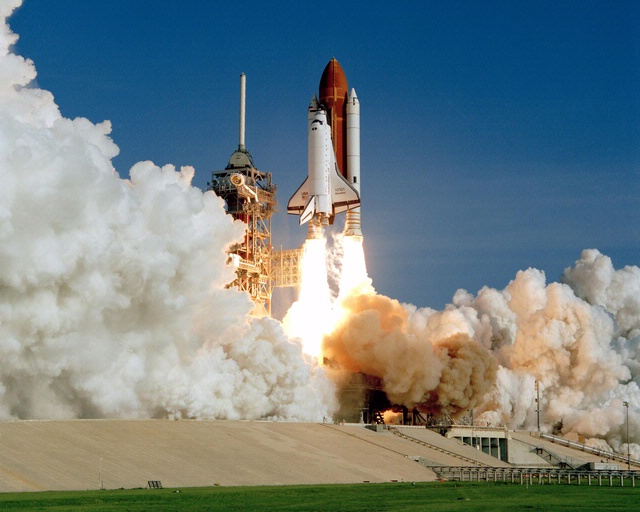
\includegraphics[scale=0.35]{gambar/roketluarangkasa.jpg}

  % Ubah dengan keterangan gambar yang diinginkan
  \caption{Peluncuran roket luar angkasa \emph{Discovery} \parencite{roketluarangkasa}.}
  \label{fig:roketluarangkasa}
\end{figure}

Roket luar angkasa merupakan \lipsum[1]

\emph{Discovery}, Gambar \ref{fig:roketluarangkasa}, merupakan \lipsum[2]

\section{Gravitasi}
\label{sec:gravitasi}

Gravitasi merupakan \lipsum[1]

\subsection{Hukum Newton}
\label{subsec:hukumnewton}

Newton \parencite{newton1687} pernah merumuskan bahwa \lipsum[1]
Kemudian menjadi persamaan seperti pada persamaan \ref{eq:hukumpertamanewton}.

% Contoh pembuatan persamaan
\begin{equation}
  \label{eq:hukumpertamanewton}
  \sum \mathbf{F} = 0\; \Leftrightarrow\; \frac{\mathrm{d} \mathbf{v} }{\mathrm{d}t} = 0.
\end{equation}

\subsection{Anti Gravitasi}
\label{subsec:antigravitasi}

Anti gravitasi merupakan \lipsum[1]

  \cleardoublepage

  % Bab 3 desain dan implementasi
  \chapter{METODOLOGI}
\label{chap:desainimplementasi}

% Ubah bagian-bagian berikut dengan isi dari desain dan implementasi

Penelitian ini dilaksanakan sesuai desain sistem berikut beserta implementasinya.
Desain sistem merupakan konsep dari pembuatan dan perancangan infrastruktur dan kemudian
diwujudkan dalam bentuk blok-blok alur yang harus dikerjakan. Pada bagian implementasi merupakan
pelaksanaan teknis untuk setiap blok pada desain sistem.

\section{Peralatan}
\label{sec:peralatan}

Peralatan yang digunakan selama pengerjaan tugas akhir ini yaitu Laptop untuk pengerjaan tugas akhir dari awal hingga penulisan buku dengan spesifikasi sebagai berikut

\section{Software}
\label{sec:software}

Sejumlah software digunakan sebagai pendukung pengerjaan Tugas Akhir ini.
Software yang berhubungan dengan Ethereum Blockchain diantaranya Remix,
Metamask, Ganache, dan Unreal Engine 5. Kemudian dari segi platform, yang digunakan adalah IPFS
dan Plugin-plugin yang ada di Unreal Engine 5 serta blueprintnya. Sementara dari Ethereum Blockchain,
bahasa pemrograman yang digunakan adalah Solidity.

% Contoh pembuatan potongan kode
\begin{lstlisting}[
  language=C++,
  caption={Program halo dunia.},
  label={lst:halodunia}
]
#include <iostream>

int main() {
    std::cout << "Halo Dunia!";
    return 0;
}
\end{lstlisting}

\subsection{Remix IDE}
Remix adalah sebuah lingkungan pengembangan (IDE) yang populer dan terbuka untuk kontrak pintar (smart contract) Ethereum yang ditulis dalam bahasa Solidity. Remix menyediakan antarmuka yang intuitif dan lengkap untuk mengedit, menguji, dan menerapkan kontrak pintar secara langsung dari browser web tanpa perlu mengunduh atau menginstal perangkat lunak tambahan.

Remix menyediakan berbagai fitur yang memudahkan pengembangan kontrak pintar dalam bahasa Solidity. Beberapa fitur utama dari Remix meliputi:

\begin{enumerate}
  \item Editor Solidity: Remix menyediakan editor Solidity yang terintegrasi, yang memungkinkan pengembang untuk menulis, mengedit, dan memeriksa sintaksis dan kesalahan dalam kontrak pintar mereka. Editor ini juga menawarkan fitur seperti penyorotan sintaksis, penjajaran otomatis, dan saran kode (code completion) untuk mempercepat pengembangan.
  \item Penjelajah File: Remix memungkinkan pengembang untuk melihat struktur proyek mereka dengan menggunakan penjelajah file terintegrasi. Pengembang dapat dengan mudah menjelajahi dan mengatur file kontrak pintar, library, dan dependensi lainnya.
  \item Pemecah Masalah (Debugger): Remix dilengkapi dengan pemecah masalah yang kuat yang memungkinkan pengembang untuk menguji dan menganalisis langkah-demi-langkah eksekusi kontrak pintar. Dengan pemecah masalah, pengembang dapat memverifikasi logika dan perilaku kontrak pintar serta menemukan dan memperbaiki bug dengan lebih efisien.
  \item Simulasi dan Uji: Remix menyediakan fitur simulasi dan pengujian yang memungkinkan pengembang untuk menjalankan dan menguji kontrak pintar dalam lingkungan virtual sebelum diterapkan di jaringan Ethereum yang sebenarnya. Fitur ini membantu pengembang untuk mengidentifikasi dan memperbaiki masalah sebelum kontrak pintar diterapkan secara nyata.
  \item Integrasi Jaringan: Remix dapat terhubung ke berbagai jaringan Ethereum, termasuk jaringan pengembangan lokal seperti Ganache atau jaringan Ethereum utama. Ini memungkinkan pengembang untuk menguji dan menerapkan kontrak pintar pada berbagai lingkungan dengan mudah.
\end{enumerate}

Remix telah menjadi salah satu alat yang sangat populer dan diandalkan dalam komunitas pengembangan Ethereum. Antarmuka yang kuat dan berfitur lengkap, serta kemudahan penggunaan langsung dari browser, menjadikan Remix sebagai pilihan favorit bagi pengembang untuk mengembangkan, menguji, dan menerapkan kontrak pintar dalam bahasa Solidity.

\begin{figure}[H]
  \centering

  % Ubah dengan nama file gambar dan ukuran yang akan digunakan
  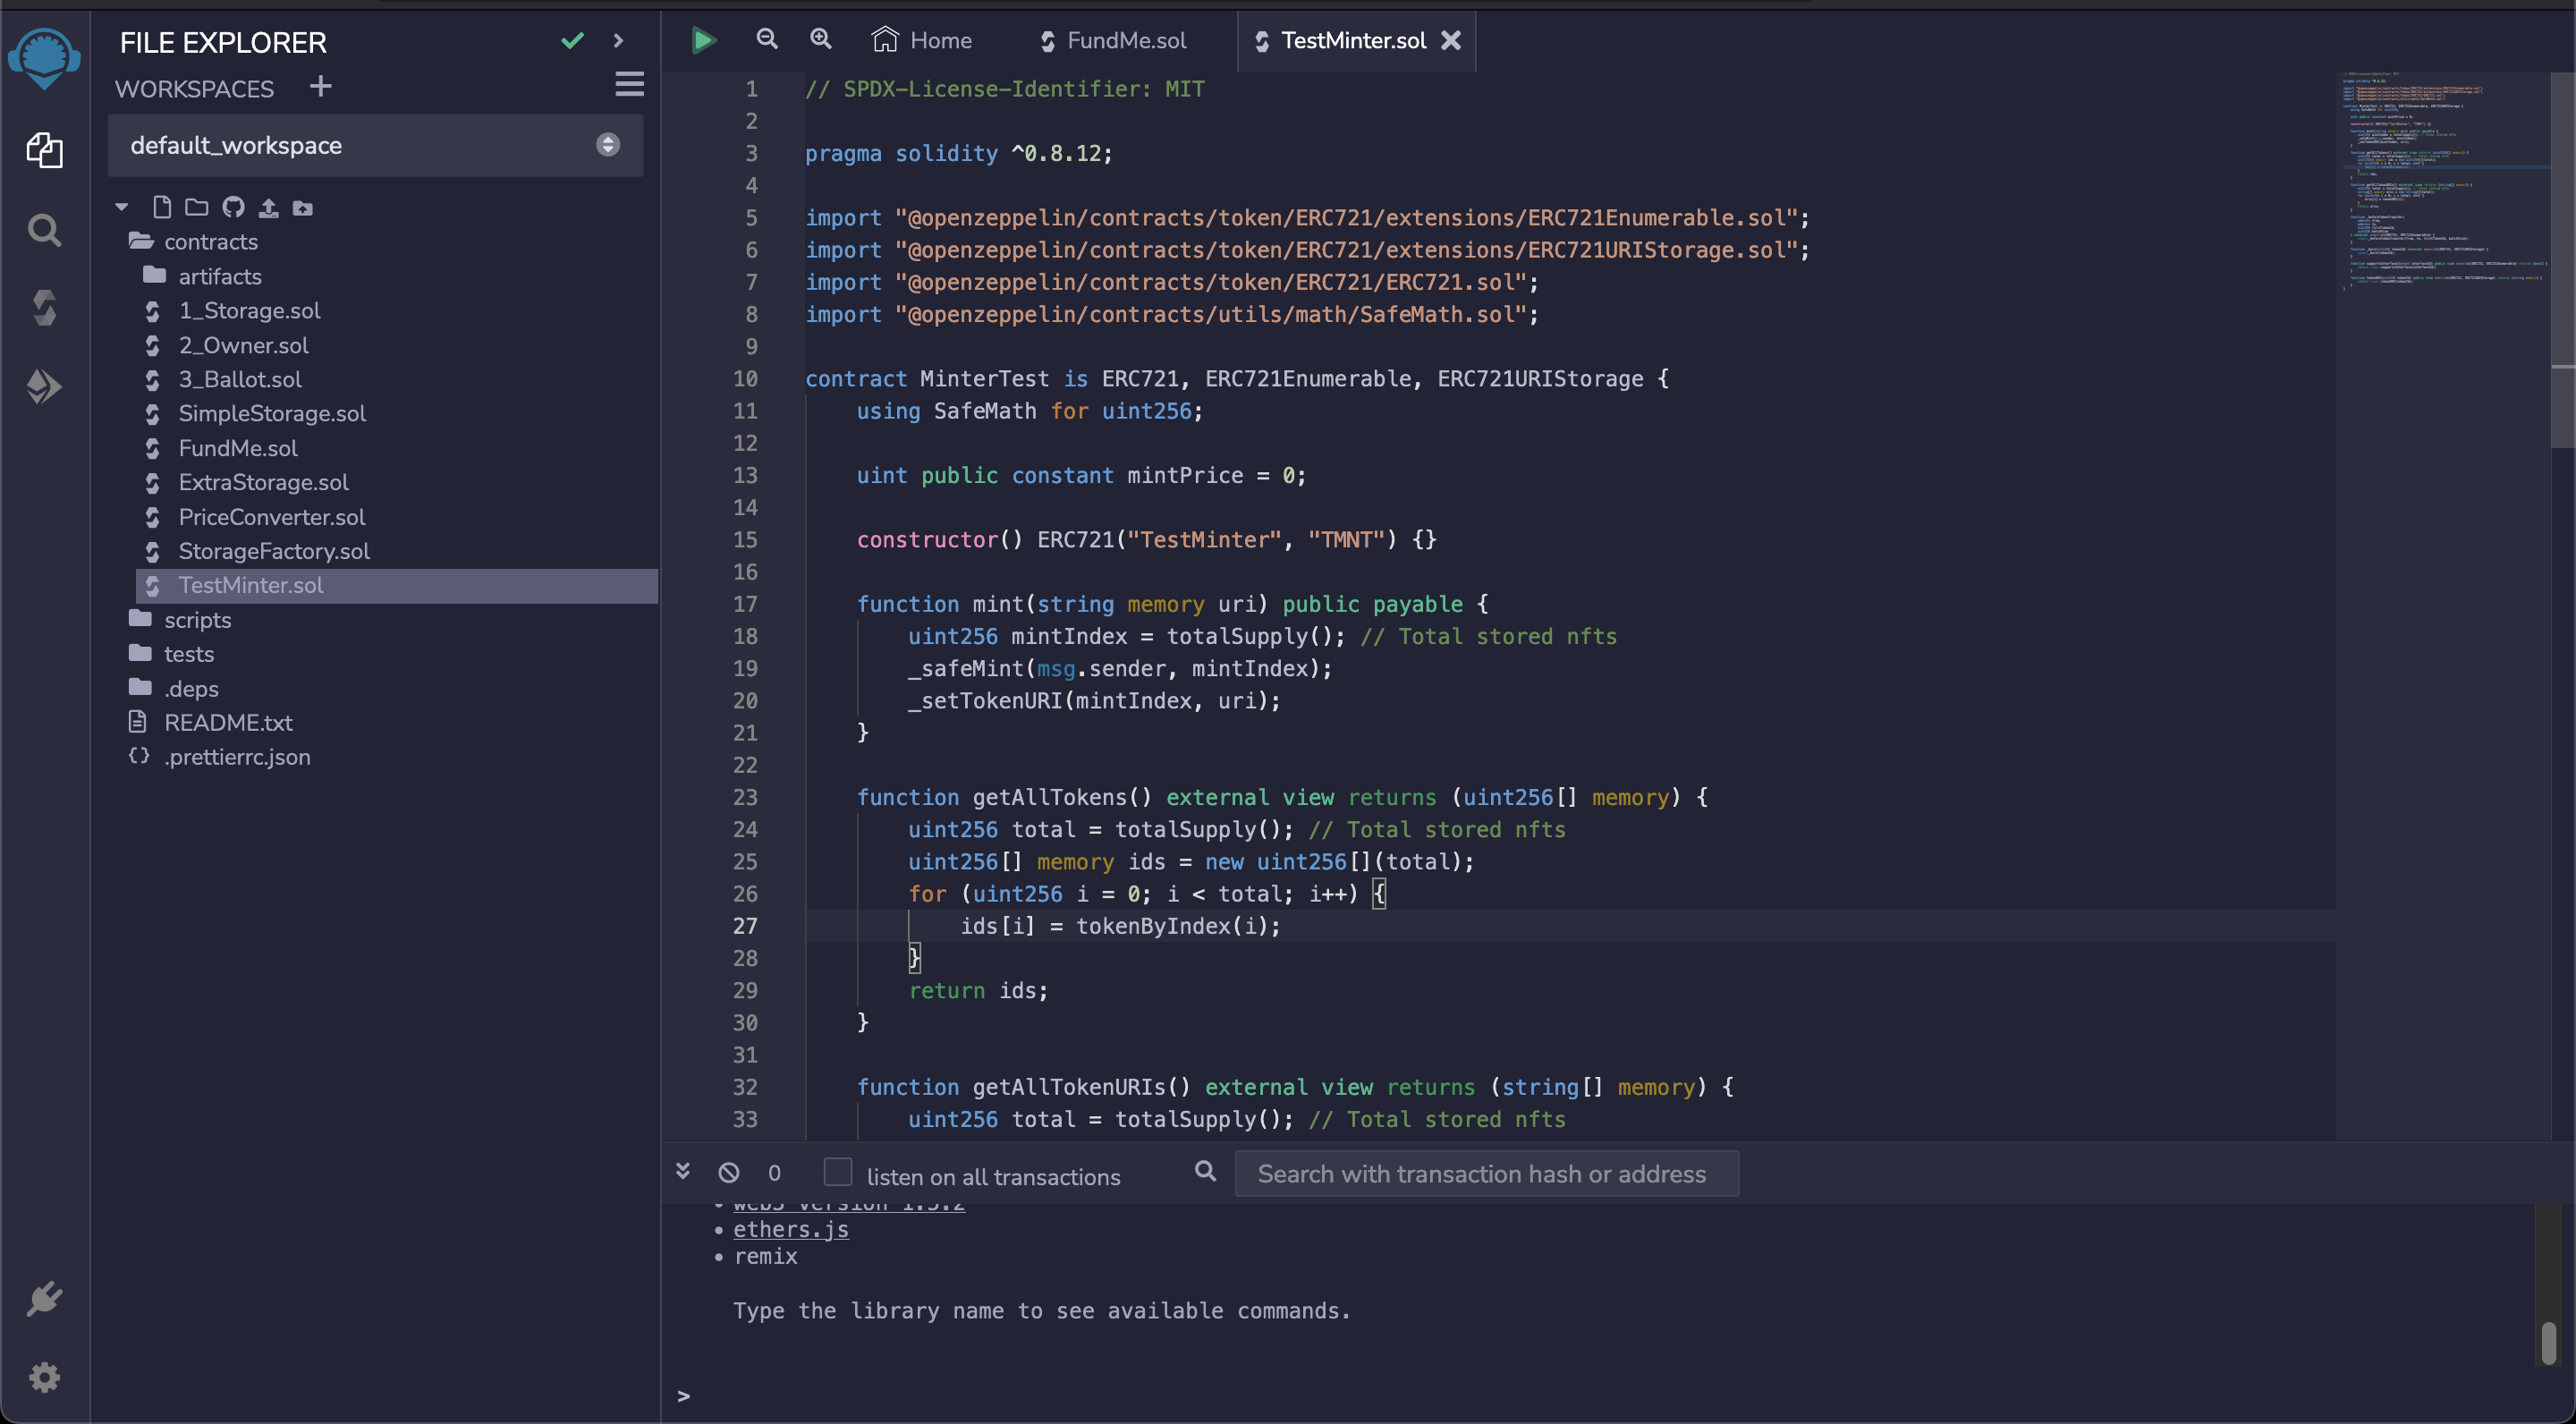
\includegraphics[scale=0.3]{gambar/remixide.png}

  % Ubah dengan keterangan gambar yang diinginkan
  \caption{Tampilan \emph{Remix IDE}.}
  \label{fig:remixide}
\end{figure}

\subsection{Ganache}
Ganache adalah sebuah perangkat lunak yang digunakan dalam pengembangan aplikasi berbasis blockchain, khususnya pada platform Ethereum. Ini adalah salah satu alat yang sangat populer di antara pengembang karena menyediakan lingkungan pengujian lokal yang mudah digunakan dan fleksibel.

Ganache awalnya dikenal dengan nama "TestRPC" sebelum berganti nama menjadi "Ganache". Perangkat lunak ini memungkinkan pengembang untuk melakukan pengembangan, pengujian, dan debugging aplikasi blockchain secara lokal tanpa perlu terhubung ke jaringan Ethereum yang sebenarnya. Dengan menggunakan Ganache, pengembang dapat membuat jaringan Ethereum pribadi mereka sendiri di mesin lokal mereka.

Berikut adalah beberapa fitur utama yang ditawarkan oleh Ganache:

\begin{enumerate}
  \item Jaringan Ethereum Lokal: Ganache menyediakan jaringan Ethereum lokal yang dapat dijalankan pada mesin pengembang. Jaringan ini berjalan di dalam lingkungan sandbox yang aman, yang memungkinkan pengembang untuk membuat dan menguji kontrak pintar, mentransaksikan token, dan menjalankan semua operasi yang terkait dengan Ethereum tanpa risiko kehilangan dana atau interaksi dengan jaringan utama.
  \item Blockchain Deterministik: Salah satu fitur kunci dari Ganache adalah kepastian (determinism) dari blockchain yang dihasilkan. Ini berarti bahwa setiap kali Ganache dijalankan dengan pengaturan yang sama, blockchain akan memiliki keadaan awal yang identik. Ini memungkinkan pengembang untuk menguji dan mengulangi skenario dengan hasil yang konsisten, yang sangat penting dalam pengujian dan debugging aplikasi blockchain.
  \item Mode Pembuatan Blok: Ganache menawarkan beberapa mode pembuatan blok yang dapat disesuaikan sesuai dengan kebutuhan pengembangan. Mode ini memungkinkan pengembang untuk mengendalikan bagaimana blok dibuat dan transaksi dikonfirmasi. Misalnya, pengembang dapat mengatur blok agar hanya dibuat setiap kali ada transaksi, atau mengatur kecepatan pembuatan blok agar sesuai dengan kecepatan transaksi yang diinginkan.
  \item Akun dan Kunci Pribadi: Ganache menyediakan sejumlah akun Ethereum yang siap digunakan dalam pengembangan. Setiap akun dilengkapi dengan kunci pribadi yang terkait, sehingga pengembang dapat menguji fungsi-fungsi yang melibatkan transaksi, seperti pengiriman Ether atau eksekusi kontrak pintar.
  \item Alat Pengembangan: Ganache dilengkapi dengan berbagai alat pengembangan yang membantu dalam memahami dan menganalisis aktivitas blockchain. Ini termasuk penjelajah blok (block explorer) yang memungkinkan pengembang untuk melihat detail transaksi dan status kontrak pintar, serta alat untuk melacak log dan debug kontrak pintar.
\end{enumerate}

Ganache dapat digunakan dalam berbagai skenario pengembangan, mulai dari pengujian kontrak pintar, pengembangan aplikasi terdesentralisasi, hingga pengujian keamanan. Dengan menggunakan Ganache, pengembang dapat dengan mudah membuat dan mengelola jaringan Ethereum lokal mereka sendiri, mempercepat siklus pengembangan, dan memastikan kualitas dan keandalan aplikasi blockchain yang dikembangkan.

\begin{figure}[H]
  \centering

  % Ubah dengan nama file gambar dan ukuran yang akan digunakan
  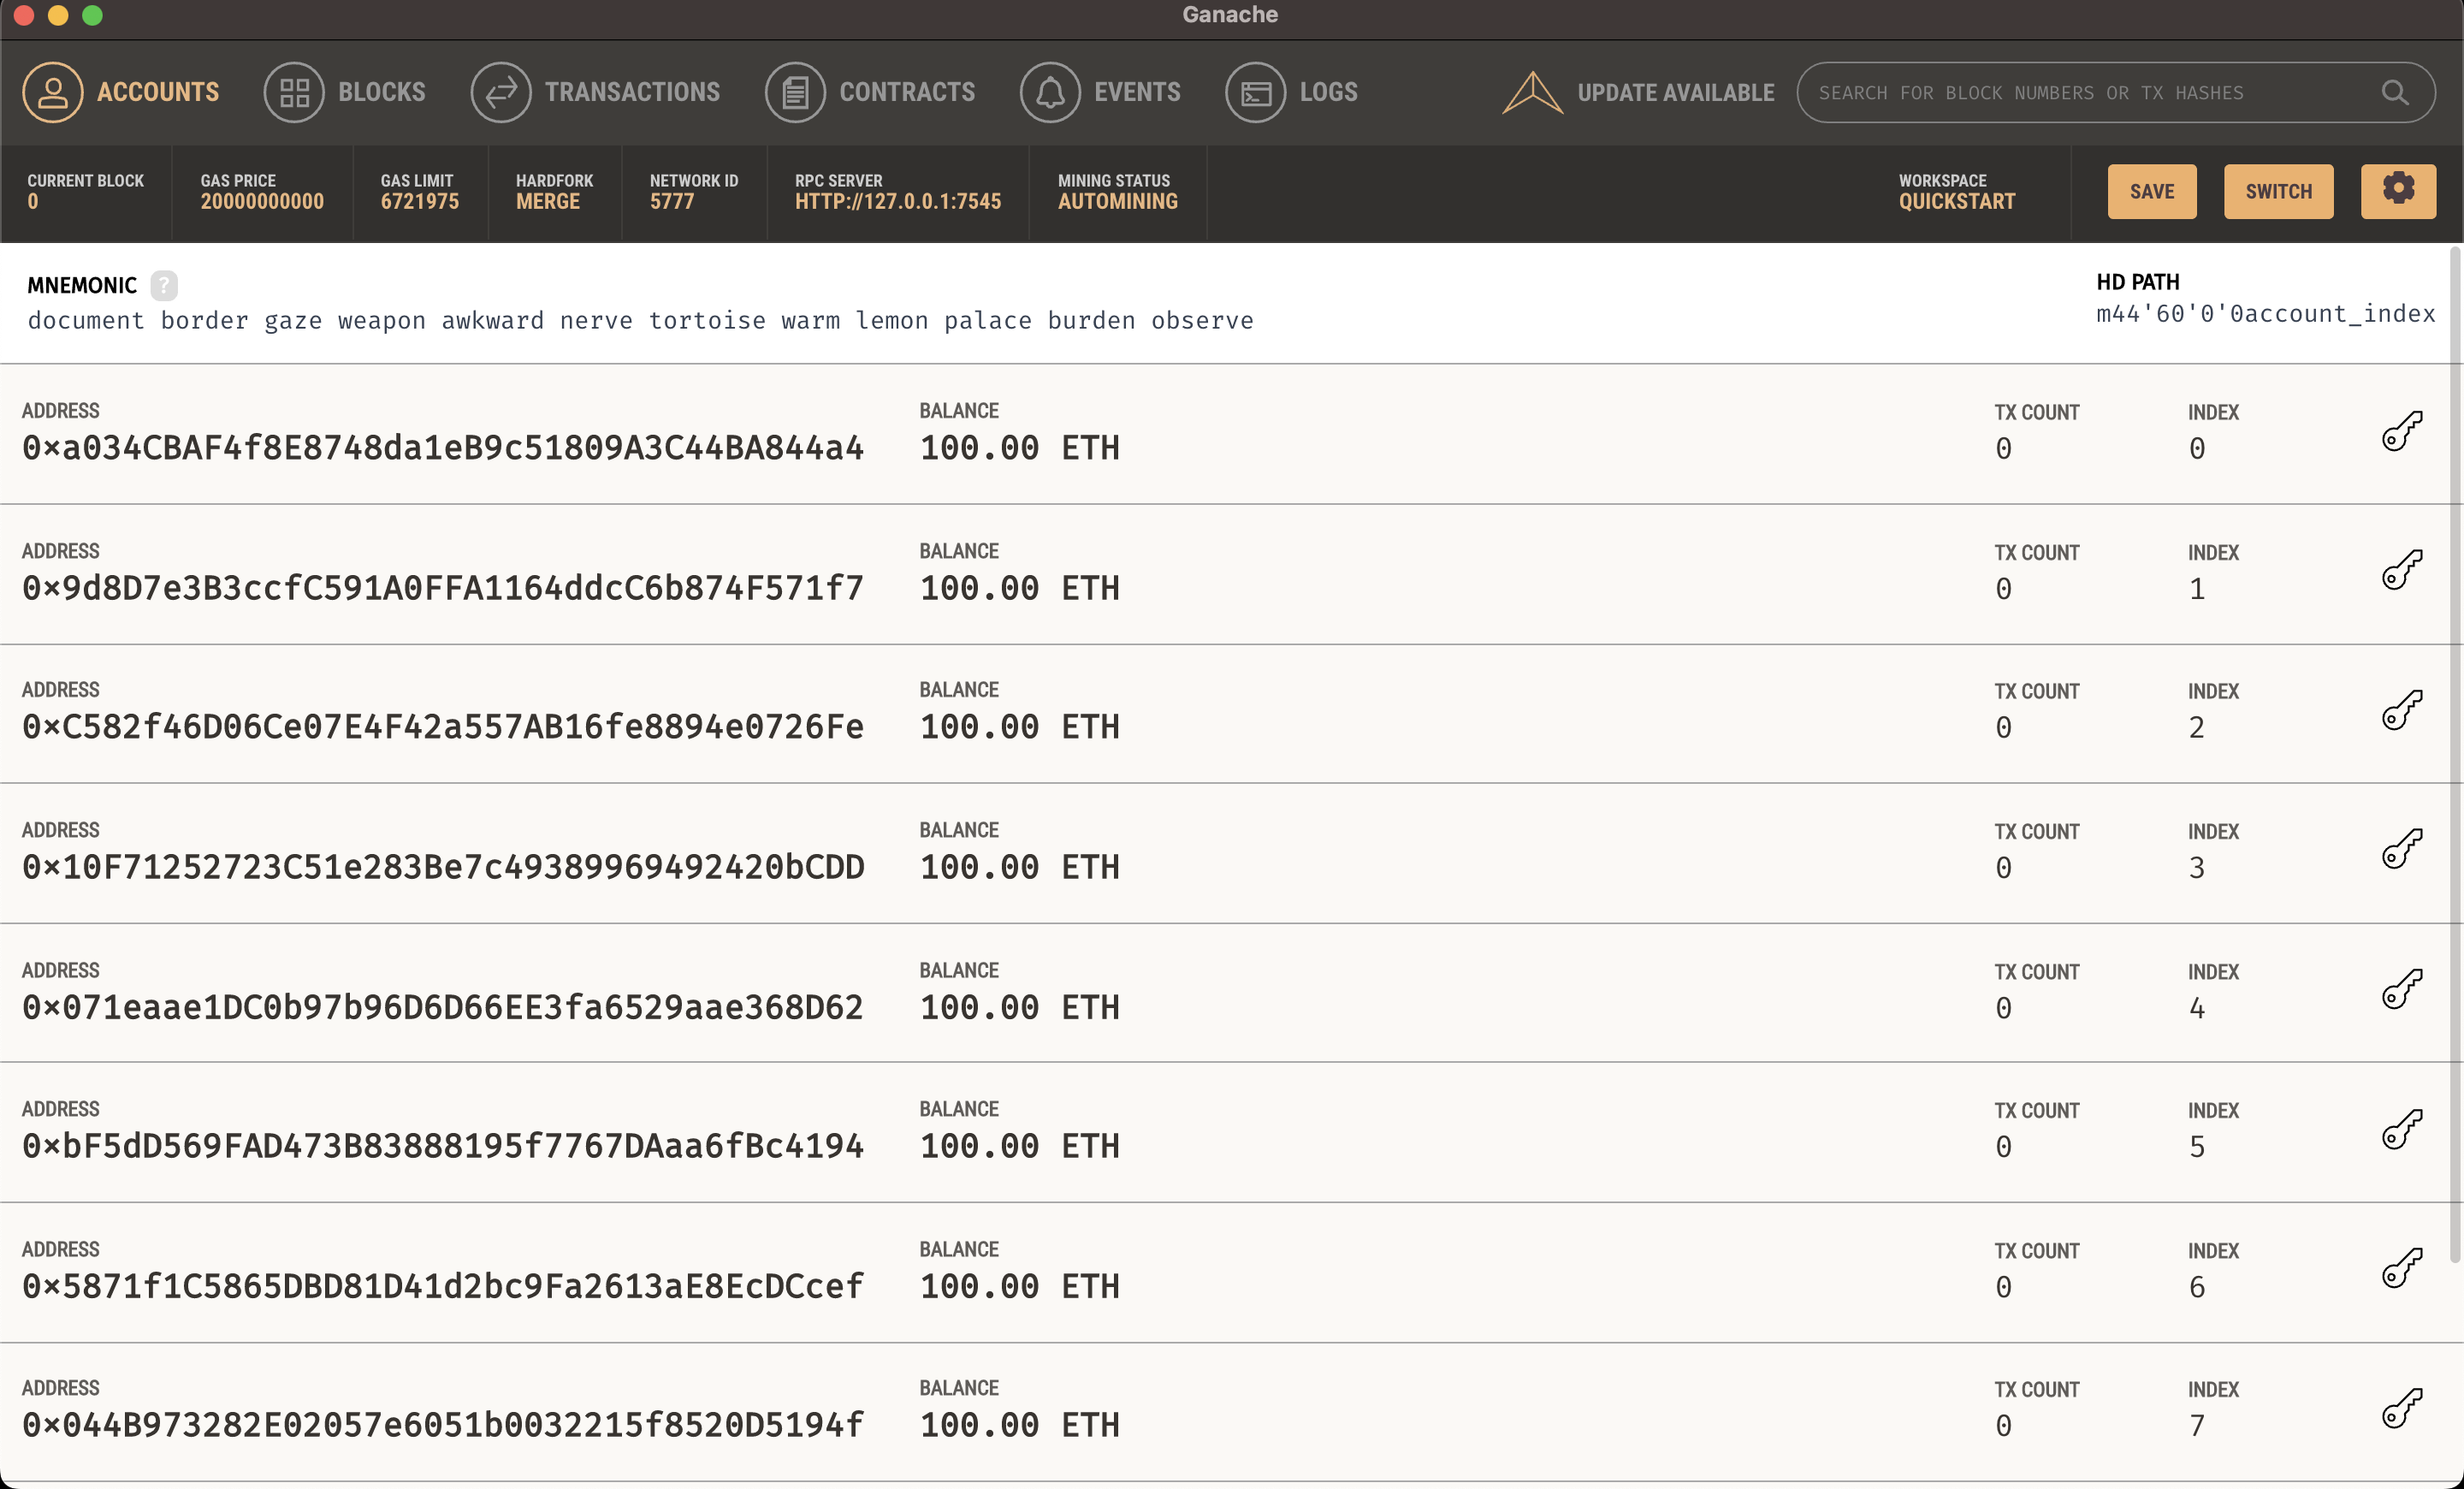
\includegraphics[scale=0.3]{gambar/ganache.png}

  % Ubah dengan keterangan gambar yang diinginkan
  \caption{Tampilan \emph{Ganache}.}
  \label{fig:ganache}
\end{figure}

\subsection{Unreal Engine 5}
Unreal Engine yang digunakan adalah versi 5.0.3. Unreal Engine digunakan untuk pengimplementasian \emph{Metaverse} yang mana dibuat sebuah lingkungan virtual sederhana seperti berikut.

\begin{figure}[H]
  \centering

  % Ubah dengan nama file gambar dan ukuran yang akan digunakan
  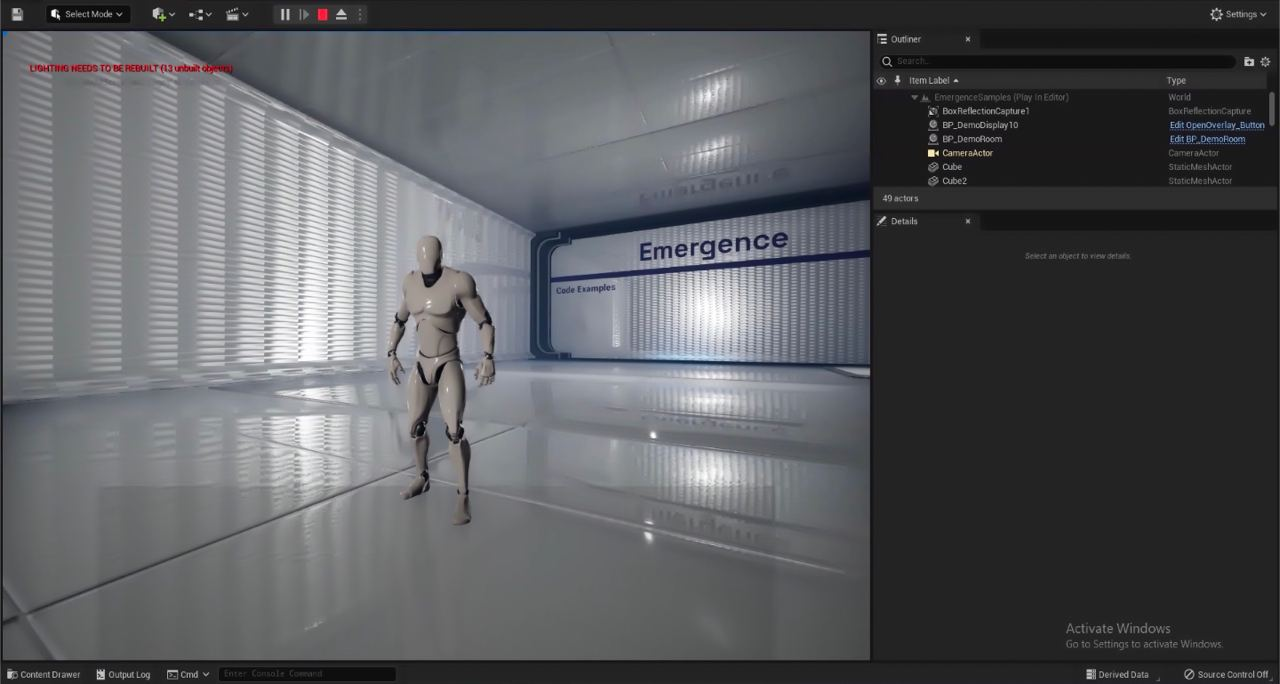
\includegraphics[scale=0.3]{gambar/ue5sample.jpg}

  % Ubah dengan keterangan gambar yang diinginkan
  \caption{Tampilan \emph{Unreal Engine 5}.}
  \label{fig:ue5sample}
\end{figure}

\section{Desain Sistem}

Tugas akhir ini dikerjakan dengan menggunakan beberapa service dan setiap service ini memiliki langkah-langkah tersendiri dalam pengerjaannya.
Untuk data \emph{raw} dari audionya disimpan di IPFS menggunakan Web3 Storage. Lalu untuk transmisi datanya menggunakan NFT yang akan di mint
dengan menggunakan protokol \emph{ERC-721}. Proses pembuatan NFT dilakukan dengan menggunakan smart contract yang ditulis dengan bahasa \emph{Solidity}

Penulisan \emph{Smart contract} dengan menggunakan \emph{solidity} dilakukan dengan menggunakan \emph{Remix IDE}.
\emph{Smart contract} yang ditulis diberikan beberapa \emph{method} tambahan yang akan membantu proses pengembangan dan integrasi ke \emph{Unreal Engine 5}

Setelah \emph{smart contract} ditulis, \emph{smart contract} dideploy. Kemudian dilakukan mint token dengan menggunakan tmapilan antarmuka dari Remix IDE.
Setelah sudah dilakukan deployment maka selanjutnya dilakukan pengintegrasian dengan Unreal Engine 5. NFT yang sudah di-mint dapat diperoleh dengan menggunakan
\emph{method smart contract} yang sudah ditulis sebelumnya. \emph{Metadata} yang tersimpan di NFT akan digunakan dan file audio yang terkandung didalamnya akan
di-play.

\begin{figure}[H]
  \centering

  % Ubah dengan nama file gambar dan ukuran yang akan digunakan
  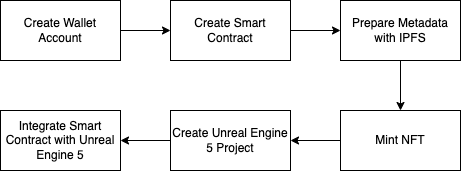
\includegraphics[scale=1]{gambar/desainsistem.png}

  % Ubah dengan keterangan gambar yang diinginkan
  \caption{Desain Sistem}
  \label{fig:desainsistem}
\end{figure}

\section{Create Wallet Account}

Proses pertama yang dilakukan adalah pembuatan akun wallet Ethereum dengan bantuan Metamask. Metamask merupakan sebuah plugin browser yang berfungsi sebagai
dompet penyimpanan Ethereum. Plugin ini dapat berinteraksi dengan Blockchain Ethereum yang didalamnya banyak terdapat aplikasi yang terdesentralisasi. Jaringan Ethereum dalam Metamask sangat beragam. Secara defaultnya, jaringan terdiri dari 2 jenis yakni Mainnet dan juga Testnet.

\begin{figure}[H]
  \centering

  % Ubah dengan nama file gambar dan ukuran yang akan digunakan
  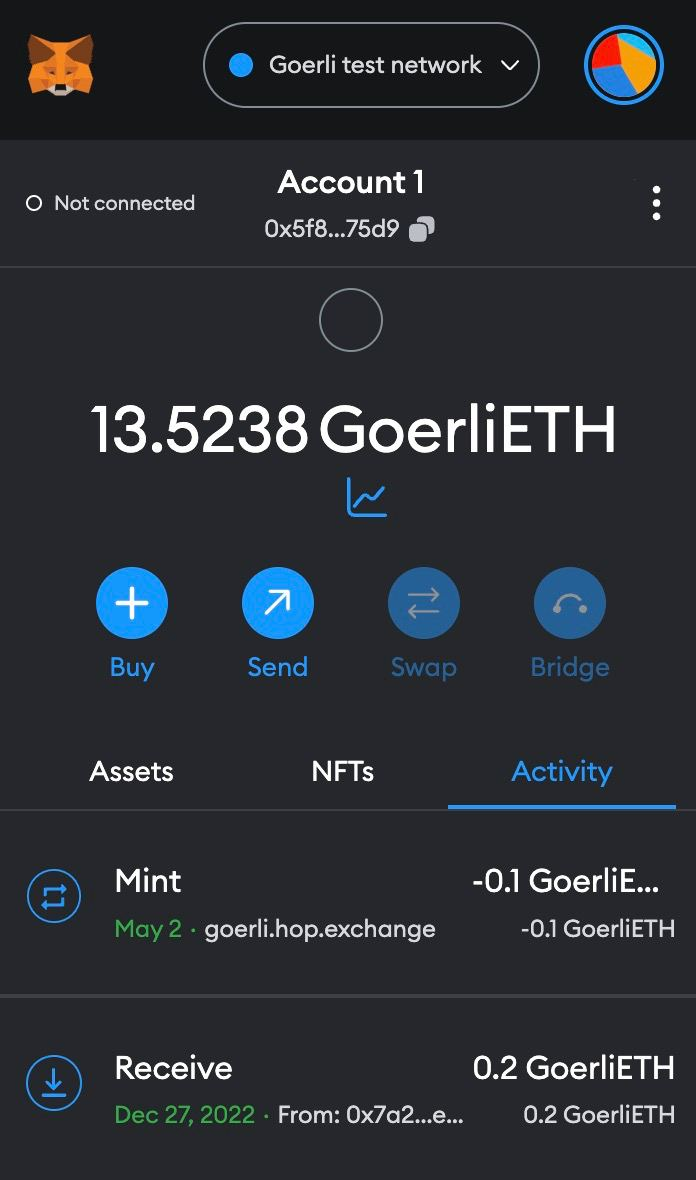
\includegraphics[scale=0.2]{gambar/tampilan-metamask.jpg}

  % Ubah dengan keterangan gambar yang diinginkan
  \caption{Tampilan Metamask}
  \label{fig:tampilanmetamask}
\end{figure}

Mainnet mengharuskan user untuk mengisi dompet Metamask dengan mata uang Ether asli, sehingga Metamask ini bisa digunakan untuk transaksi sehari-hari melewati jaringan Mainnet ini.
Sedangkan jaringan Testnet merupakan jaringan berbentuk perco- baan yang biasa digunakan untuk pengembangan aplikasi yang ingin diintegrasikan dengan Metamask. Pilihan Testnet ini juga tidak hanya satu, melainkan defaultnya terdapat
4 jaringan Testnet dalam Metamask, antara lain Ropsten, Goerli, Kovan, dan Rinkeby.

Masing-masing Testnet ini memiliki algoritma konsensus seperti Proof of Work dan Proof of Authority. Ropsten Testnet menggunakan algoritma Proof of Work dan Testnet lainnya menggunakan Proof of Authority. Untuk Proof of Stake dalam default plugin Metamask belum tersedia, namun Testnet dengan algoritma ini sudah tersedia seperti Kiln dan Kitsugi, dapat ditambahkan jaringannya pada Metamask.

Setelah membuat akun, akan diberikan Secret Recovery Phrase yang merupakan 12 kata unik dari Metamask sebagai cadangan untuk bisa masuk ke akun Metamask ketika password untuk login terlupakan. Secret Recovery Phrase ini dianjurkan untuk tidak disebarkan karena pengguna lain yang tidak memiliki akses ke password bisa mengakses akun Metamask orang lain hanya dengan Recovery Secret Phrase. Dalam plugin Metamask, pengguna dibebaskan membuat sejumlah akun lewat jaringan manapun. Untuk project ini, digunakan Testnet Ropsten yang menganut algoritma Proof of Work serta jaringan lokal Blockchain yang diperoleh dari Ganache sebagai mata uang untuk pengujian Smart Contract dan aplikasi.

Pada tahap ini, akun Testnet secara default akan memiliki 0 Ether, namun akun tersebut dapat memperoleh Ether dengan mencari faucet dari Testnet nya. Faucet ini nantinya yang akan mengirimkan sejumlah Ether sehingga akun Testnet bisa memperoleh Ether tanpa melakukan komputasi apapun. Maka dengan demikian, akun ini dinamakan Externally Owned Account, yang bisa dikendalikan langsung oleh pengguna tanpa perlu dikaitkan program. Nominal Testnet yang didapat hasil dari faucet bisa dikirimkan lang- sung ke akun lain di Testnet yang sama dengan fitur transfer between account, inilah fitur yang menjelaskan Externally Owned Account (EOA).

\begin{figure}[H]
  \centering

  % Ubah dengan nama file gambar dan ukuran yang akan digunakan
  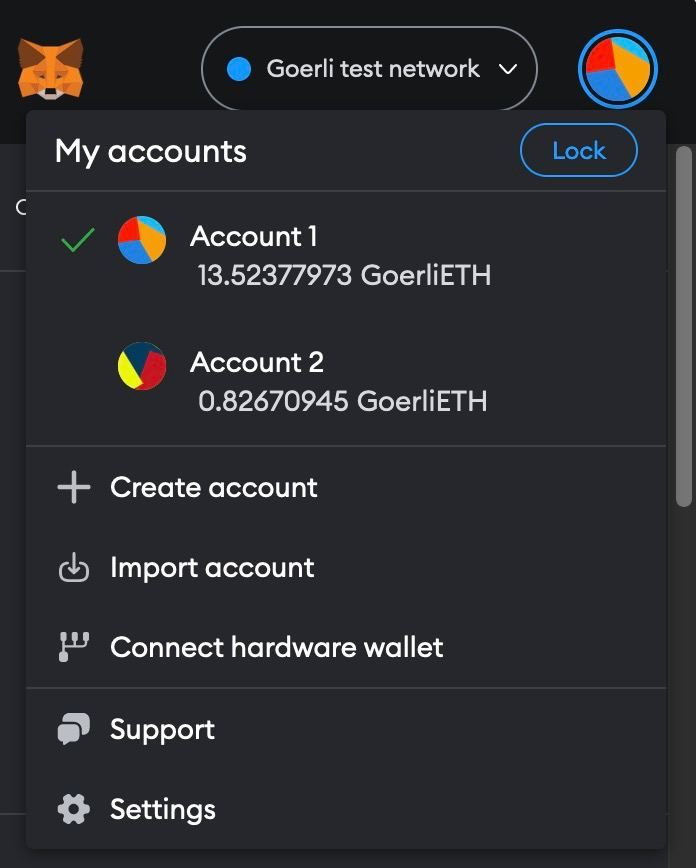
\includegraphics[scale=0.2]{gambar/akun-goerli.jpg}

  % Ubah dengan keterangan gambar yang diinginkan
  \caption{Tampilan Akun Goerli di Metamask}
  \label{fig:akungoerli}
\end{figure}

Akun wallet dari Metamask ini merupakan Ethereum Account yang dibuat dari kriptografis private dan public key. Dengan private key, membantu membuktikan bahwa transaksi benar-benar ditandatangani oleh pengirim dan mencegah pemalsuan. Public key dalam Metamask berarti sama dengan walllet address dari akun token Testnet yang digunakan (biasanya berawal dari 0x). Karena account Ethereum ini membutuhkan private
key untuk menandatangi transaksi agar bisa dikonfirmasi pada ledger, maka dari itu sistem ini menggunakan jenis yang sama pada sistem Multi Signature yaitu menggunakan 2 atau lebih private key untuk menandatangi transaksi dari akun yang berbeda. Komparasi dengan sistem wallet di Indonesia saat ini menunjukan perbedaan dimana di Indonesia, sistemnya saat ini menggunakan 2 factor authentication dengna OTP dan juga PIN untuk melakukan transaksi sehingga media nya berbeda. Tetapi pada sistem layanan uang digital di Indonesia masih bersifat sentralisasi, sedangkan pada Multi Signature karena memanfaatkan teknologi Blockchain Ethereum, bersifat desentralisasi. Pada implementasinya, Multi Signature dapat menggunakan prinsip 2FA dengan cara menggunakan device yang berbeda. Satu orang dapat mengimplementasikan sistem ini jika memiliki lebih dari satu device untuk melakukan koneksi ke wallet yang sudah memiliki sistem Multi Signature

\section{Create \emph{Smart Contract}}

Pembuatan Smart Contract merupakan salah satu kelebihan dari Ethereum, dimana fitur didalam wallet Ether semua diprogram dalam Smart Contract sesuai dengan kebutuhan.
Token yang akan digunakan adalah token dengan spesifikasi ERC-721 atau disebut juga dengan NFT (Non Fungible Token)
Pertama ditentukan spesifikasi token ERC-721 yang ingin dibuat. Ini meliputi pengaturan seperti nama token, simbol, dan jumlah total token yang akan dikeluarkan.
Dapat juga dipertimbangkan apakah perlu menyertakan metadata tambahan seperti deskripsi, gambar, atau atribut khusus.
Kontrak pintar (smart contract) harus dibuat menggunakan bahasa pemrograman Solidity dengan library standar ERC-721 diimpor dan kontrak didefinisikan sebagai kontrak yang mengimplementasikan interface ERC-721.
Fungsi-fungsi utama seperti transfer token, melihat informasi token, dan lainnya perlu diatur. Logika bisnis yang diinginkan perlu diimplementasikan pada token ERC-721. Uji dan rilis harus dilakukan untuk memastikan kontrak berfungsi sebagaimana yang diharapkan.
Kontrak dapat diuji secara lokal menggunakan alat pengujian seperti Ganache atau Remix sebelum dirilis ke jaringan Ethereum.

Dalam smart contract yang dibuat, diberikan method-method tambahan seperti \texttt{tokenURI}, \texttt{getAllTokens}, dan \texttt{getAllTokenURIs}.

% Contoh input potongan kode dari file
\lstinputlisting[
  language=Solidity,
  caption={Smart Contract untuk Mint NFT.},
  label={lst:bilanganprima}
]{program/TestMinter.sol}

Listing diatas adalah kontrak smart contract Solidity yang menggunakan beberapa kontrak dari library OpenZeppelin untuk mengimplementasikan ERC-721, ERC-721Enumerable, dan ERC-721URIStorage. Berikut adalah pembahasan secara lebih rinci setiap bagian dari kode tersebut:

\subsection{Kontrak Import dan Inheritance}
Kontrak menggunakan @openzeppelin/contracts library untuk mengimpor kontrak ERC721, ERC721Enumerable, dan ERC721URIStorage. Kontrak MinterTest adalah turunan dari ketiga kontrak tersebut.
\subsection{Konstruktor}
Konstruktor digunakan untuk menginisialisasi kontrak dengan memberikan nama dan simbol untuk token ERC-721 yang dibuat.
Dalam kode ini, konstruktor didefinisikan menggunakan fungsi constructor() dengan menggunakan konstruktor kontrak ERC721.

\subsection{Fungsi Mint}
Fungsi mint digunakan untuk membuat token baru dan meng-assign kepemilikannya kepada pengirim transaksi.
Fungsi ini menerima parameter uri yang merupakan URI unik untuk token yang akan dibuat.
Setelah token dibuat, fungsi \_safeMint digunakan untuk mengalokasikan token kepada pengirim transaksi.
Fungsi \_setTokenURI digunakan untuk mengatur URI token.

\subsection{Fungsi getAllTokens}
Fungsi getAllTokens digunakan untuk mengembalikan array dengan daftar semua token yang ada dalam kontrak.
Fungsi ini menggunakan fungsi totalSupply untuk mendapatkan total jumlah token yang ada.
Kemudian, dalam loop, fungsi tokenByIndex digunakan untuk mendapatkan ID token pada indeks tertentu.

\subsection{Fungsi getAllTokenURIs}
Fungsi getAllTokenURIs digunakan untuk mengembalikan array dengan daftar URI semua token dalam kontrak.
Fungsi ini juga menggunakan fungsi totalSupply untuk mendapatkan total jumlah token yang ada.
Dalam loop, fungsi tokenURI digunakan untuk mendapatkan URI token pada indeks tertentu.

\subsection{Fungsi \_beforeTokenTransfer dan \_burn}
Fungsi \_beforeTokenTransfer dan \_burn merupakan fungsi internal yang di-override dari kontrak ERC721 dan ERC721URIStorage.
Fungsi \_beforeTokenTransfer dijalankan sebelum token transfer terjadi.
Fungsi \_burn dijalankan saat token di-burn (dihapus) dari kontrak.

\subsection{Fungsi supportsInterface dan tokenURI}
Fungsi supportsInterface dan tokenURI adalah fungsi yang di-override dari kontrak ERC721 dan ERC721URIStorage.
Fungsi supportsInterface memeriksa apakah kontrak mendukung interface tertentu.
Fungsi tokenURI mengembalikan URI token berdasarkan ID token yang diberikan.

Setelah dilakukan penulisan kode solidity maka dapat dilakukan deployment. Deployment dilakukan dengan environment \emph{Injected Provider - Metamask}


\begin{figure}[H]
  \centering

  % Ubah dengan nama file gambar dan ukuran yang akan digunakan
  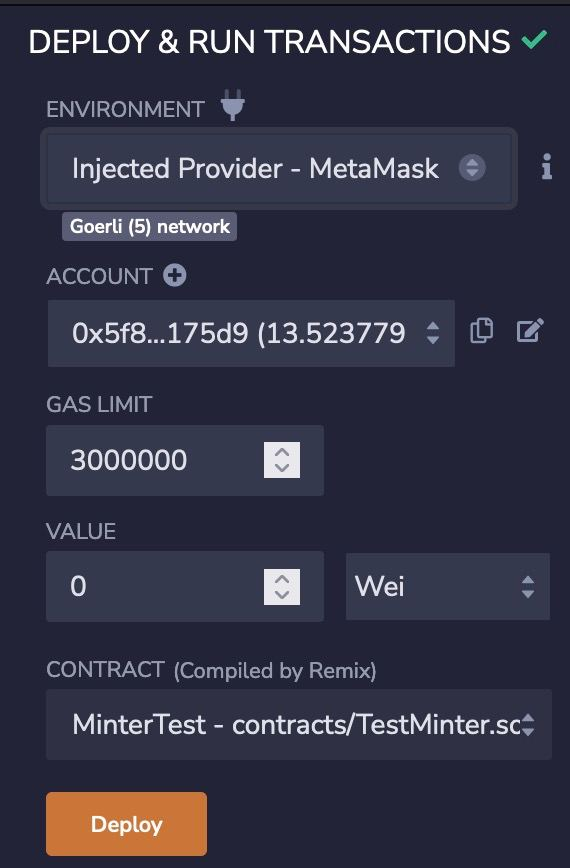
\includegraphics[scale=0.4]{gambar/deployment-interface.jpg}

  % Ubah dengan keterangan gambar yang diinginkan
  \caption{Antarmuka Deployment di Remix IDE}
  \label{fig:deploymentinterface}
\end{figure}

\section{Prepare Metadata with IPFS}

Untuk melakukan persiapan metadata, maka perlu ditentukan dulu format JSON yang akan digunakan. Format JSON yang digunakan adalah format dari
OpenSea yang adalah seperti berikut.


\begin{figure}[H]
  \centering

  % Ubah dengan nama file gambar dan ukuran yang akan digunakan
  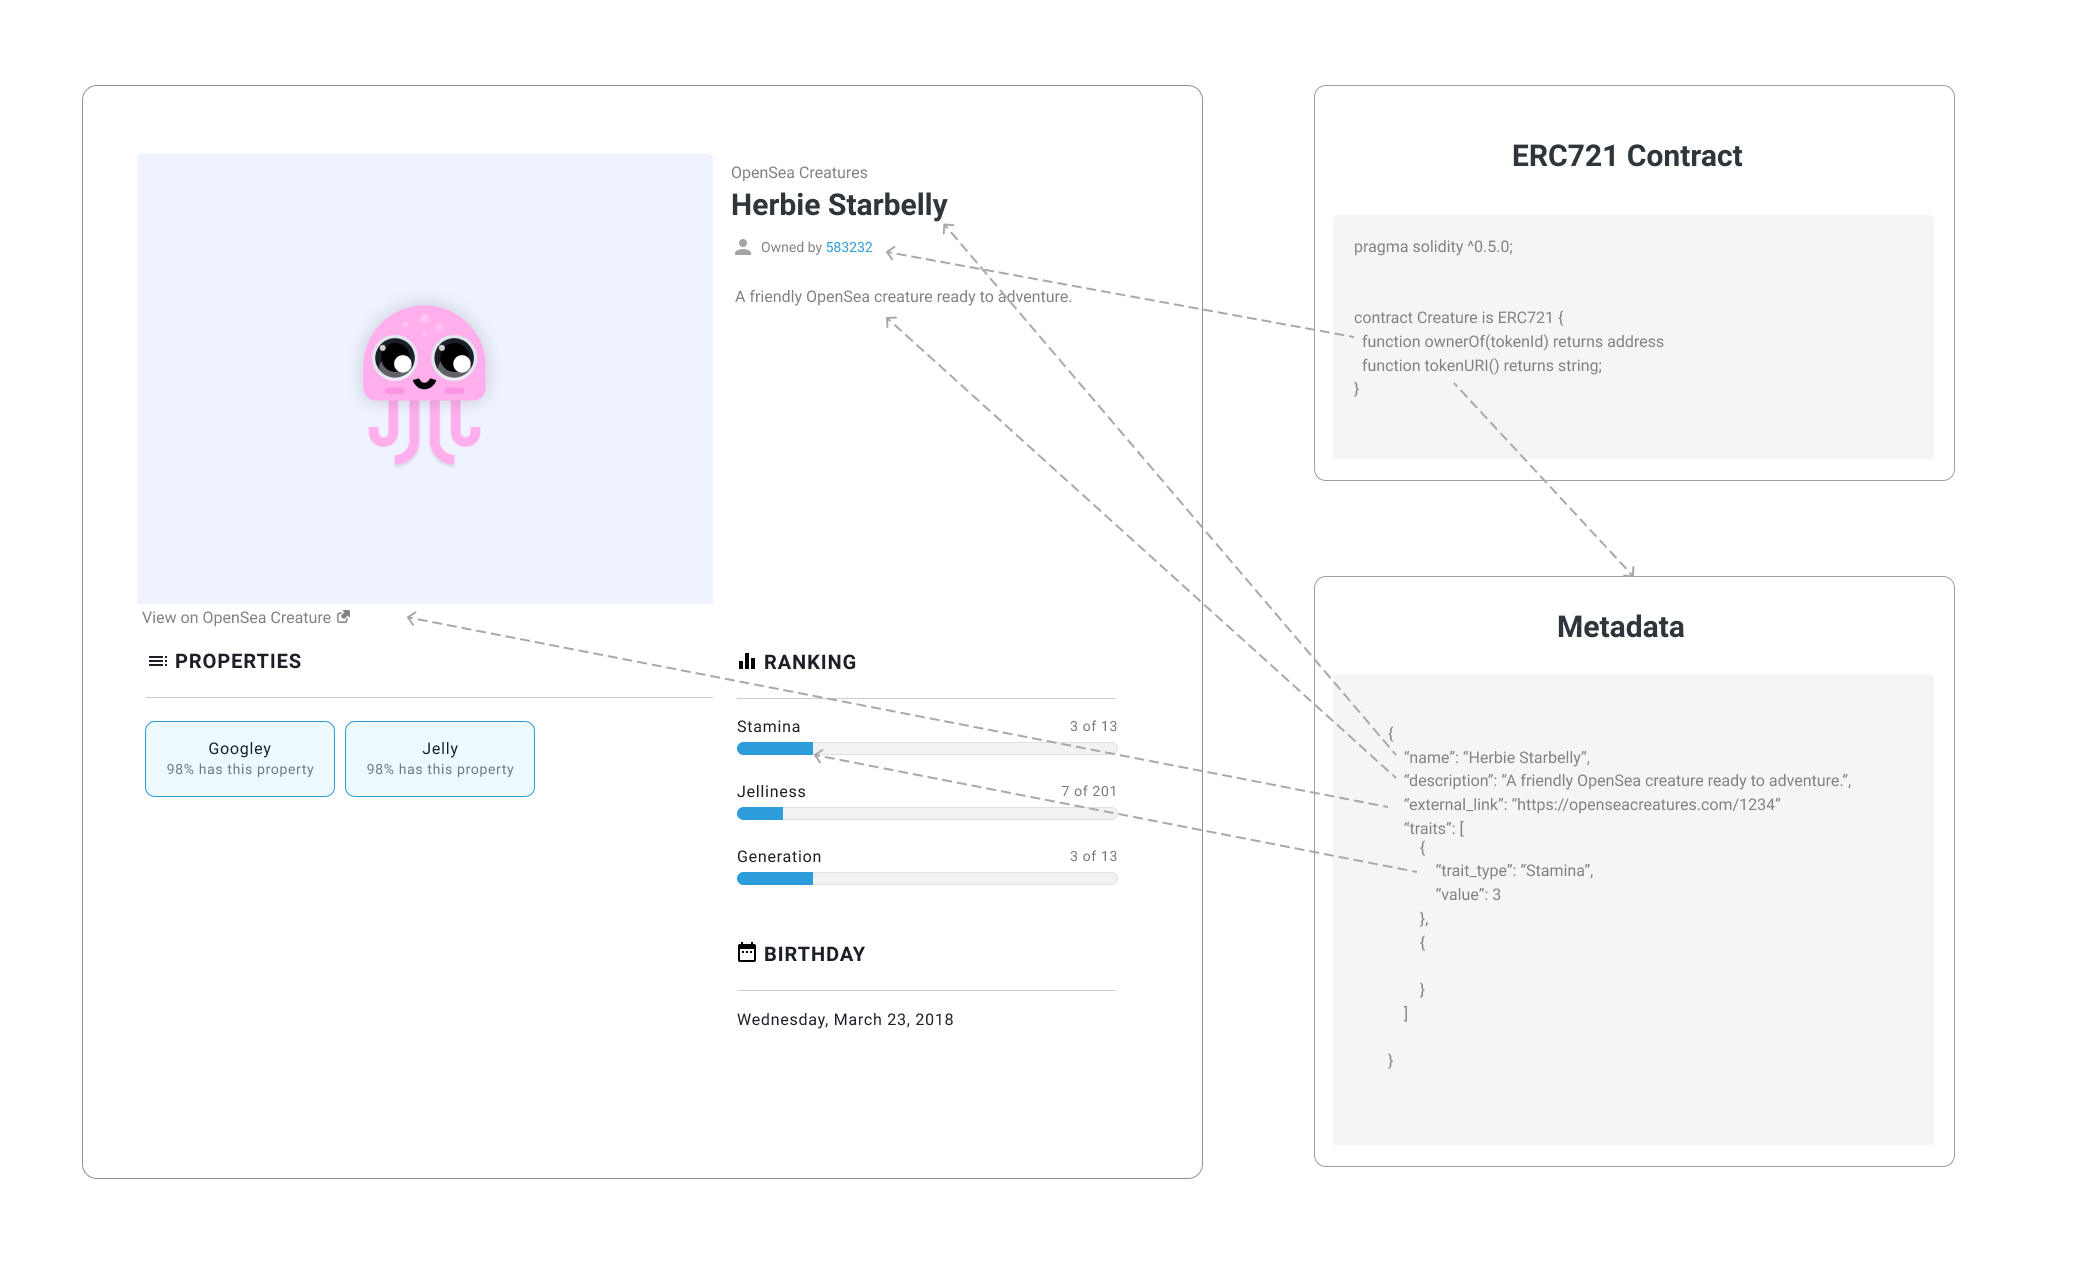
\includegraphics[scale=0.23]{gambar/nft-standards-opensea.png}

  % Ubah dengan keterangan gambar yang diinginkan
  \caption{Standar NFT OpenSea}
  \label{fig:openseanft}
\end{figure}

Dari struktur metadata tersebut, dibuatlah beberapa modifikasi dan tambahan field seperti audio\_url untuk menampung URL dari audio yang digunakan.
\lstinputlisting[
  language=json,
  caption={Format JSON untuk metadata NFT.},
  label={lst:nftformat}
]{program/nft-1.json}

\subsection{Web3 Storage}
Service IPFS yang digunakan adalah Web3 Storage. Semua asset-asset yang akan digunakan diunggah di Web3 Storage.

web3.storage adalah kumpulan API dan layanan yang memudahkan pengembang dan pengguna lain untuk berinteraksi dengan data tanpa terikat pada lokasi fisik penyimpanan data tersebut. Layanan ini secara asli menggunakan protokol data dan identitas terdesentralisasi seperti IPFS, Filecoin, dan UCAN yang memungkinkan arsitektur dan alur kerja aplikasi yang berfokus pada verifikasi data dan pengguna.

Di inti platform ini terdapat layanan penyimpanan terhosting yang dapat digunakan untuk mengunggah dan menyimpan data agar tetap tersedia secara berkelanjutan. Platform ini juga menyediakan layanan tambahan seperti w3link dan w3name yang memudahkan pembuatan pengalaman web yang mulus dan menyenangkan dengan memanfaatkan protokol web3.

\begin{figure}[H]
  \centering

  % Ubah dengan nama file gambar dan ukuran yang akan digunakan
  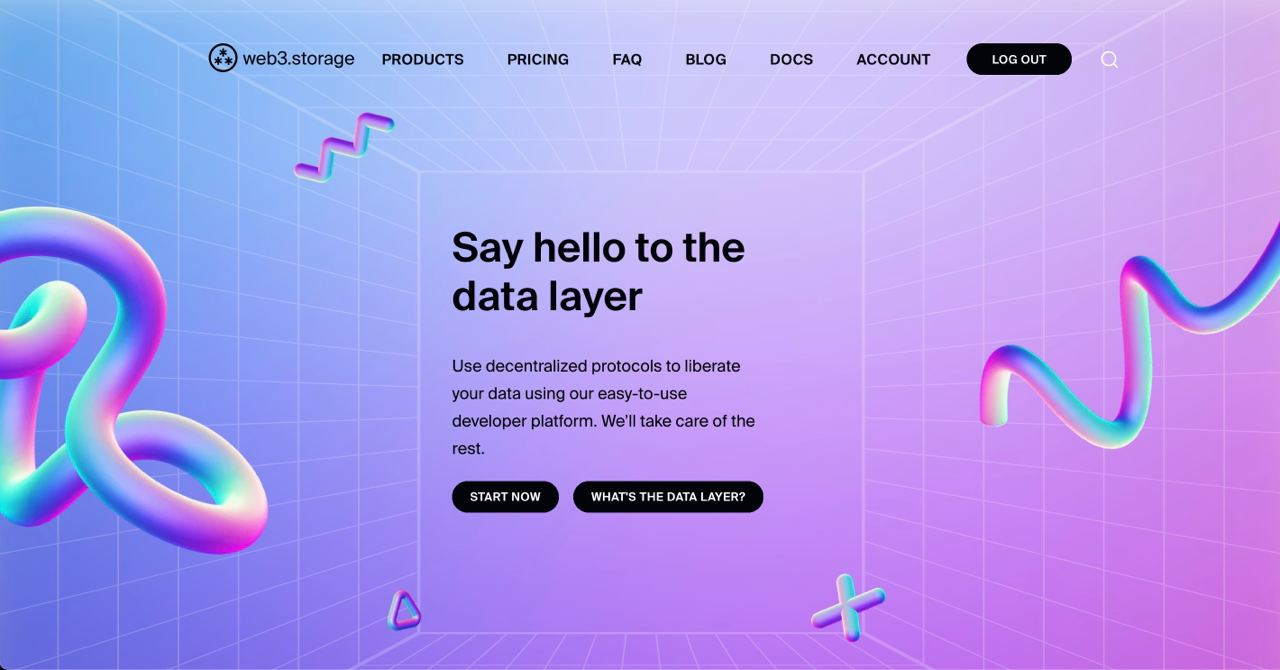
\includegraphics[scale=0.3]{gambar/web3storage.jpg}

  % Ubah dengan keterangan gambar yang diinginkan
  \caption{Tampilan web3.storage}
  \label{fig:web3storage}
\end{figure}

Dengan menggunakan web3.storage akan diupload file-file yang akan digunakan untuk data dari sistem.
Data-data atau assets ini menggunakan audio yang berlisensi CC0.

\begin{figure}[H]
  \centering

  % Ubah dengan nama file gambar dan ukuran yang akan digunakan
  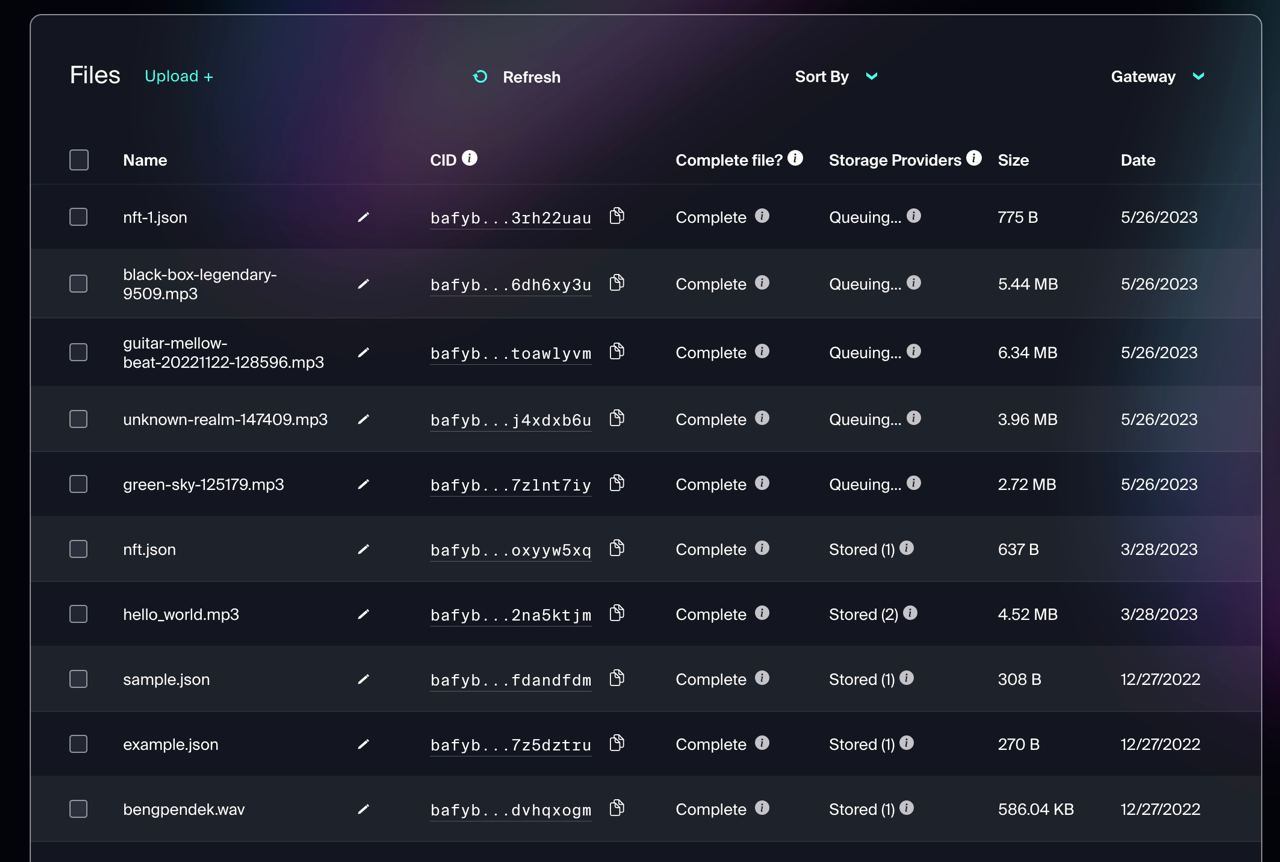
\includegraphics[scale=0.3]{gambar/web3storageacc.jpg}

  % Ubah dengan keterangan gambar yang diinginkan
  \caption{Tampilan di menu file web3.storage}
  \label{fig:web3storageacc}
\end{figure}

Url dari audio yang sudah diupload akan diletakkan kedalam Metadata json, kemudian json tersebut akan diupload juga
ke web3.storage.

\section{Mint NFT}

  \cleardoublepage

  % Bab 4 pengujian dan analisis
  \chapter{PENGUJIAN DAN ANALISIS}
\label{chap:pengujiananalisis}

% Ubah bagian-bagian berikut dengan isi dari pengujian dan analisis

Pada penelitian ini dipaparkan \lipsum[1][1-5]

\section{Skenario Pengujian}
\label{sec:skenariopengujian}

Pengujian dilakukan dengan \lipsum[1-2]

\section{Evaluasi Pengujian}
\label{sec:analisispengujian}

Dari pengujian yang \lipsum[1]

% Contoh pembuatan tabel
\begin{longtable}{|c|c|c|}
  \caption{Hasil Pengukuran Energi dan Kecepatan}
  \label{tb:EnergiKecepatan}\\
  \hline
  \rowcolor[HTML]{C0C0C0}
  \textbf{Energi} & \textbf{Jarak Tempuh} & \textbf{Kecepatan} \\
  \hline
  10 J & 1000 M & 200 M/s \\
  20 J & 2000 M & 400 M/s \\
  30 J & 4000 M & 800 M/s \\
  40 J & 8000 M & 1600 M/s \\
  \hline
\end{longtable}

\lipsum[2-4]

  \cleardoublepage

  % Bab 5 penutup
  \chapter{PENUTUP}
\label{chap:penutup}

% Ubah bagian-bagian berikut dengan isi dari penutup

\section{Kesimpulan}
\label{sec:kesimpulan}

Berdasarkan hasil pengujian yang mulai dari pengujian sistem Sharing Data Audio berbasis blockchain pada Smart Contract hingga integrasi unreal engine 5, diperoleh beberapa kesimpulan sebagai berikut:

\begin{enumerate}[nolistsep]

  \item Kode \emph{Smart contract} yang dibuat memiliki kompleksitas yang terukur oleh konsumsi gas sebesar 3275354 unit \emph{gas} untuk melakukan \emph{deployment smart contract} di \emph{testnet}, dan 3274368 di \emph{Ganache}. Untuk pemanggilan \emph{method mint} memiliki kompleksitas yang terukur sebesar 125574 unit \emph{gas} di \emph{testnet}

  \item Sistem ini memiliki beberapa ketentuan format yang mengikat mengingat pada pengujian diperlukan data yang valid pada \emph{JSON metadata}, yang memiliki setidaknya 1 \emph{key} \texttt{audio\_url}.

  \item Sinergi untuk web3 tercapai dengan adanya integrasi dengan smart contract ethereum yang juga interoperable dengan blockchain lain seperti solana dan polygon.

  \item Terdapat 3 file audio yang dapat dibaca oleh Unreal Engine 5 secara real time, yakni mp3, flac, dan wav.

\end{enumerate}

\section{Saran}
\label{chap:saran}

Untuk pengembangan lebih lanjut pada penelitian ini, terdapat beberapa saran yang bisa dilakukan khususnya pada sistem data sharing berbasis blockchain ini, yang mana diantara lain:

\begin{enumerate}[nolistsep]

  \item Menggunakan \emph{metasound} pada versi Unreal Engine 5.3 yang akan datang karena akan semakin erat kaitannya dengan web3 dan metaverse. Pada penelitian ini menggunakan audio player bawaan dari Unreal Engine 5.

  \item Membuat sistem validasi yang lebih \emph{robust} sehingga dapat mencegah error runtime baik pada smart contract dan juga Unreal Engine 5 terkhusus pada bagian blueprint.

  \item Membuat support yang lebih pada beberapa format audio maupun format metadata yang lebih fleksibel sehingga mempermudah baik pengembang maupun pengguna.

\end{enumerate}

  \cleardoublepage

  \chapter*{DAFTAR PUSTAKA}
  \addcontentsline{toc}{chapter}{DAFTAR PUSTAKA}
  \renewcommand\refname{}
  \vspace{2ex}
  \renewcommand{\bibname}{}
  \begingroup
  \def\chapter*#1{}
  \printbibliography
  \endgroup
  \cleardoublepage

  % Biografi penulis
  \begin{center}
  \Large
  \textbf{BIOGRAFI PENULIS}
\end{center}

\addcontentsline{toc}{chapter}{BIOGRAFI PENULIS}

\vspace{2ex}

\begin{wrapfigure}{L}{0.3\textwidth}
  \centering
  \vspace{-3ex}
  % Ubah file gambar berikut dengan file foto dari mahasiswa
  
\includegraphics[width=0.3\textwidth]{gambar/elon.jpg}
  \vspace{-4ex}
\end{wrapfigure}

% Ubah kalimat berikut dengan biografi dari mahasiswa
\name{} adalah seorang penulis dan pengembang perangkat lunak yang lahir di Surabaya pada tanggal 8 Desember 2001. Penulis menyelesaikan pendidikannya di Institut Teknologi Sepuluh Nopember, dengan mengambil jurusan Teknik Komputer.
Sejak awal masa studinya, penulis telah menunjukkan minat dan keahlian yang besar dalam bidang pengembangan perangkat lunak. Penulis aktif terlibat dalam berbagai kegiatan di kampus, termasuk menjadi anggota panitpenulis dalam acara MAGE 6 dan MAGE 7, yang merupakan acara besar dalam dunpenulis komputer dan teknologi.
Ketertarikan penulis terutama terfokus pada pengembangan backend dan aplikasi. Penulis memiliki pemahaman yang mendalam tentang berbagai bahasa pemrograman dan kerangka kerja yang digunakan dalam pengembangan perangkat lunak modern. Keahliannya dalam backend development memungkinkan penulis untuk mengembangkan sistem yang kuat dan efisien.
Selain itu, penulis juga memiliki ketertarikan khusus dalam topik blockchain. Dalam tugas akhirnya, penulis memilih untuk fokus pada penelitian dan pengembangan blockchain, sebuah teknologi yang memiliki potensi untuk merevolusi berbagai sektor, termasuk keuangan dan logistik.
Dalam perjalanan penulisannya, penulis telah menghasilkan berbagai artikel dan tulisan teknis terkait dengan bidang pengembangan perangkat lunak. Penulis memiliki kemampuan komunikasi yang baik dan mampu menyampaikan ide-idenya dengan jelas dan terstruktur.
Sebagai seorang yang berdedikasi dan bersemangat, penulis terus mengembangkan keterampilan dan pengetahuannya dalam industri teknologi yang terus berkembang. Penulis selalu berusaha untuk mengikuti perkembangan terbaru dalam dunpenulis pengembangan perangkat lunak dan mengaplikasikannya dalam pekerjaannya.
Jika Anda ingin menghubungi penulis, Anda dapat menghubungi melalui email di me@aaronct.dev. Penulis sangat terbuka untuk kolaborasi dan diskusi terkait dengan pengembangan perangkat lunak dan topik terkait lainnya.

  \cleardoublepage

\end{document}
